\documentclass[aspectratio=169,xcolor=dvipsnames]{beamer}
\usepackage[algo2e]{algorithm2e}
\usepackage{changepage}
\setbeamertemplate{footline}[frame number]
\setlength\tabcolsep{2pt}
\usepackage{url}
\usepackage{graphicx}
\usepackage{textpos}
\usepackage{tabulary}
\usepackage{color, colortbl}
\usepackage{tikz}

\newcolumntype{K}[1]{>{\centering\arraybackslash}p{#1}}

\definecolor{chlorine}{RGB}{161,198,63}
\definecolor{darkgreen}{RGB}{26,128,63}

\title{\ \\\ \\\ \\\ \\\textcolor{chlorine}{Machine Learning Basics}}
\author{\textcolor{darkgreen}{Mladen Nikoli\'c}\\\ \\\textcolor{darkgreen}{Machine Learning Group} \\\textcolor{darkgreen}{\url{machinelearning.math.rs}}\\\ \\\textcolor{darkgreen}{Faculty of Mathematics}\\ \textcolor{darkgreen}{University of Belgrade}}
\date{}

\begin{document}
\AtBeginSection{
\frame{
\frametitle{Overview}
\tableofcontents[currentsection]
}
}

\usebackgroundtemplate{
\includegraphics[width=\paperwidth,height=\paperheight]{title_slide.jpg}
}

\frame{
\titlepage
}

\usebackgroundtemplate{
\includegraphics[width=\paperwidth,height=\paperheight]{regular_slide.jpg}
}

\frame{
\frametitle{Overview}
\tableofcontents
}


\section{About machine learning}
\frame{
\frametitle{What is machine learning?}
\begin{itemize}
\item A discipline which deals with inducing algorithms from the data, instead of programming them explicitly
\end{itemize}
}

\frame{
\frametitle{Critical notions}
\begin{itemize}
\item Instead of algorithms, we talk about {\em models}
\item Models express relations between different {\em variables} relevant for the task being solved
\item Models are obtained from available {\em data} by some {\em learning algorithm}
\item Models should {\em generalize} well, meaning that they should perform well on {\em unseen data}
\end{itemize}
}


\frame{
\frametitle{Toy example (1)}
\begin{itemize}
\item Automated detection of computer related articles
\item How to detect them?
\item<2> Based on terminology
\item<2> For instance ''computer`` and ''file``
\item<2> Each article can be represented by frequencies of these words
\item<2> Points in 2D space!
\item<2> How to express discrimination rule between computer related ones and the others?
\end{itemize}
}

\frame{
\frametitle{Toy example (2)}
\vspace{1mm}
\begin{figure}
\input{clanci.tkz}
\hspace{3mm}
\input{razdvajanje.tkz}
\caption{P. Jani\v ci\'c, M. Nikoli\'c, Artificial intelligence, in preparation.}
\end{figure}
}


\frame{
\frametitle{Why is machine learning important?}
\begin{itemize}
\item Numerous applications which move boundaries of technology and imagination
\item Superhuman performance in some tasks (with a grain of salt)
\item Deep theory of inductive inference
\item Great interplay of theory and practice, of academia and industry
\item Most important branch of artificial intelligence
\item Probably most popular and fastest growing branch of computer science
\end{itemize}
}


\frame{
\frametitle{Machine learning and artificial intelligence}
\begin{itemize}
\item DL $\subsetneq$ ML $\subsetneq$ AI
\item Logic based AI vs. probability based AI
\item Logic formalizes deductive inference
\item ML formalizes inductive inference
\item Logic based approaches to AI expect formal definitions of inference rules and are applied to problems for which we are able to provide full formal descriptions
\item ML aims at problems for which we can't provide formal descriptions (e.g., face recognition), but can provide examples instead
\item Logic based approaches do not operate with uncertainty, while ML approach does (which is often great, but sometimes not)
\end{itemize}
}

\frame{
\frametitle{Machine learning and data mining}
\begin{itemize}
\item Data mining focuses on finding patterns (i.e., knowledge) in data
\item Almost always it includes application of machine learning algorithms
\item It also includes various steps of data preparation, exploration, model interpretation, etc.
\item Machine learning focuses on design and properties of algorithms which are able to generalize and the way those properties depend on design choices
\end{itemize}
}

\frame{
\frametitle{Machine learning and statistics}
\begin{itemize}
\item Difference is more about emphasis and culture, than in fundamental goals
\begin{itemize}
\item Major emphasis on prediction, not so much on interpretability of models
\item Major emphasis on small sample theory, not so much on asymptotics
\item More complex and powerful models and less understanding (both of the models and of the phenomenon modelled)
\item Strong emphasis on optimization and algorithmics
\item Stronger emphasis on empirical evaluation, not so much on theoretical estimates, formal properties (e.g., unbiasedness, minimal variance, etc.)
\item Provides strong theory of generalization\footnote{\hspace{1cm}Which is named ''statistical``, by the way.}
\end{itemize}
\item How about we stop drawing boundaries?
\end{itemize}
}

\frame{
\frametitle{Short history (1)}
\begin{itemize}
\item 1943 -- McCulloch and Pitts formulate threshold logic, first artificial neuron
\item 1950 -- Alan Turing contemplates about learning machines
\item 1950 -- Marvin Minsky builds a first neural network
\item 1952 -- Arthur Samuel makes first checkers playing programme
\item 1957 -- Frank Rosenblatt makes perceptron (in hardware)
\item 1963 -- Vapnik and Chervonenkis propose first support vector machine
\end{itemize}
}

\frame{
\frametitle{Short history (2)}
\begin{itemize}
\item 1967 -- Cover and Hart propose $k$ nearest neighbours algorithm with application to travelling salesman problem
\item 1969 -- Marvin Minsky and Seymor Papert criticize perceptron, leading to first neural network winter
\item 1975 -- Werbos formulates backpropagation algorithm
\item 1981 -- Dejong introduces explanation based learning for extraction of rules from data
\item 1986 -- Rumelhart, Hinton, and Williams reintroduce backpropagation
\end{itemize}
}

\frame{
\frametitle{Short history (3)}
\begin{itemize}
\item 1989 -- Watkins proposes Q-learning
\item 1989 -- First selfdriving car
\item 1992 -- Boser, Guyon, and Vapnik propose to use kernles with SVM, starting the domination of SVM during nineties
\item 1992 -- Tesauro makes TD-Gammon, backgammon system which beats human champions
\item 1995 -- Tin Kam Ho proposes random decision forests
\item 1997 -- Hochreiter and Schmidhuber propose LSTM
\end{itemize}
}


\frame{
\frametitle{Short history (4)}
\begin{itemize}
\item 2006 -- Hinton rebrands neural networks as {\em deep learning}
\item 2011 -- IBM's system Watson outcompetes human champions in Jeopardy!
\item 2012 -- Google Brain develops a system which can recognize cats in YouTube videos!!
\item 2012 -- AlexNet sets machine learning as a standard in computer vision
\item 2016 -- Google's Alpha Go defeats human world champion in the game of Go
\item 2017 -- Microsoft's speech recognition system beats human standard
\end{itemize}
}

\frame{
\frametitle{Current day applications}
\begin{minipage}{0.49\textwidth}
\begin{itemize}
\item Algorithmic trading
\item Bioinformatics
\item Brain-machine interfaces
\item Cheminformatics
\item Computer vision
\item Credit card fraud detection
\item Computer vision
\item Handwriting recognition
\item Information retrieval
\end{itemize}
\end{minipage}
\begin{minipage}{0.49\textwidth}
\begin{itemize}
\item Marketing
\item Medical diagnostics
\item Natural language processing
\item Online advertising
\item Recommender systems
\item Robot control
\item Social network analysis
\item Speech recognition
\item Tracking patient's health condition
\end{itemize}
\end{minipage}
}


\frame{
\frametitle{Analysis of images and videos}
\begin{minipage}{0.33\textwidth}
\begin{itemize}
\item Face recognition
\item Object recognition
\item 3D reconstruction
\end{itemize}
\end{minipage}
\begin{minipage}{0.66\textwidth}
\begin{figure}
\vspace{2mm}
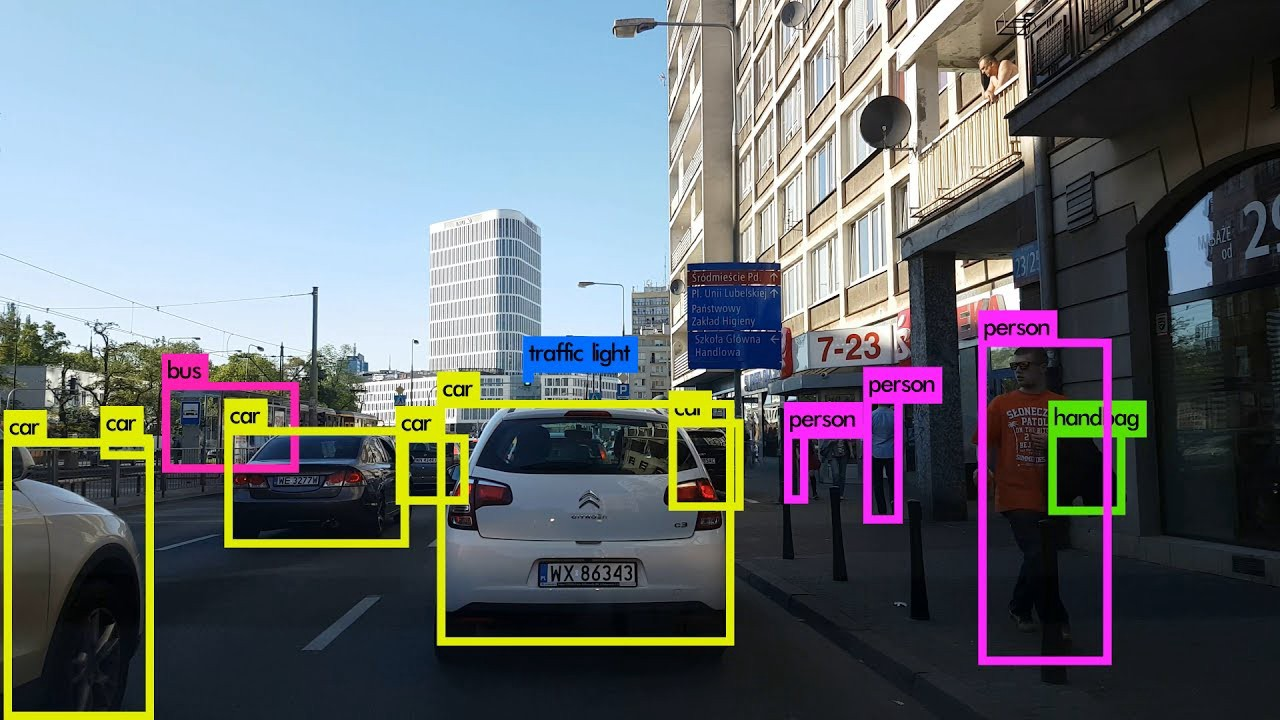
\includegraphics[width=0.9\textwidth]{yolo.jpg}
\caption{\url{https://towardsdatascience.com/yolo-v3-object-detection-53fb7d3bfe6b}}
\end{figure}
\end{minipage}
}

\frame{
\frametitle{Autonomous driving/flight}
\begin{itemize}
\item ALVINN drove 140km at the highway at the end of eighties with no human assistence
\item In the past decade numerous companies started working on autonomous vehicle driving using neural networks, reinforcement learning...
\item Autonomous flight of quadrotors, helicopters...
\end{itemize}
}

\frame{
\frametitle{Game playing}
\begin{itemize}
\item Human level backgammon player at the end of eighties
\item Alfa Go defeats human champion in Go 4 to 1
\item Neural network plays Atari games
\item Neural network plays 3D shooters (e.g., Doom) better than humans
\end{itemize}
}

\frame{
\frametitle{Natural language processing and speech recognition}
\begin{minipage}{0.49\textwidth}
\begin{itemize}
\item OCR and hand written text recognition
\item Text classification
\item Sentiment analysis
\item Topic analysis
\item Machine translation
\item Speech recognition
\item Dialog and recommendation systems
\end{itemize}
\end{minipage}
\begin{minipage}{0.49\textwidth}
\begin{figure}
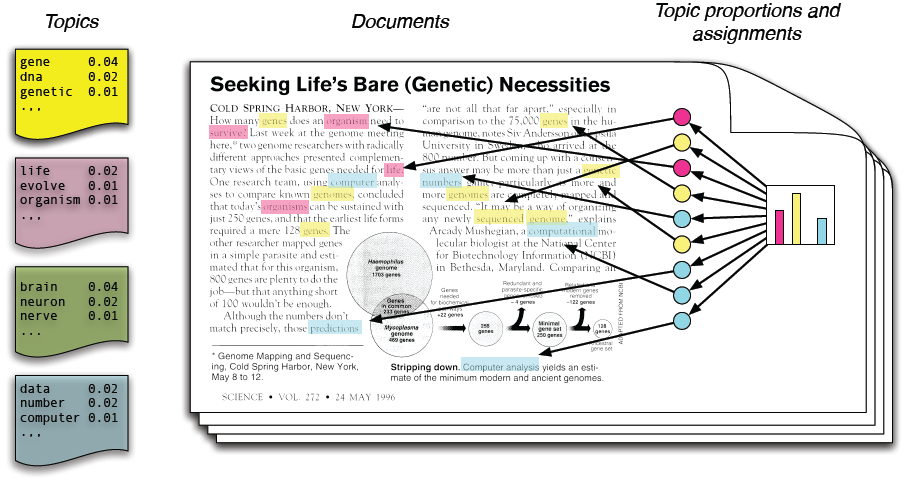
\includegraphics[width=\textwidth]{topic.png}
\caption{\url{https://rpubs.com/rain10241/63854}}
\end{figure}
\end{minipage}
}

\frame{
\frametitle{Medical applications}
\begin{itemize}
\item Tumor recognition and classification
\item Predicting patient's future health state
\item Therapy optimization (e.g., sepsis)
\end{itemize}
}

\frame{
\frametitle{Social network analysis}
\begin{minipage}{0.55\textwidth}
\begin{itemize}
\item Community detection
\item Link recommendation in social networks
\item Link detection in criminal and terrorist networks
\item Targeted advertising
\end{itemize}
\end{minipage}
\begin{minipage}{0.44\textwidth}
\vspace{3mm}
\begin{figure}
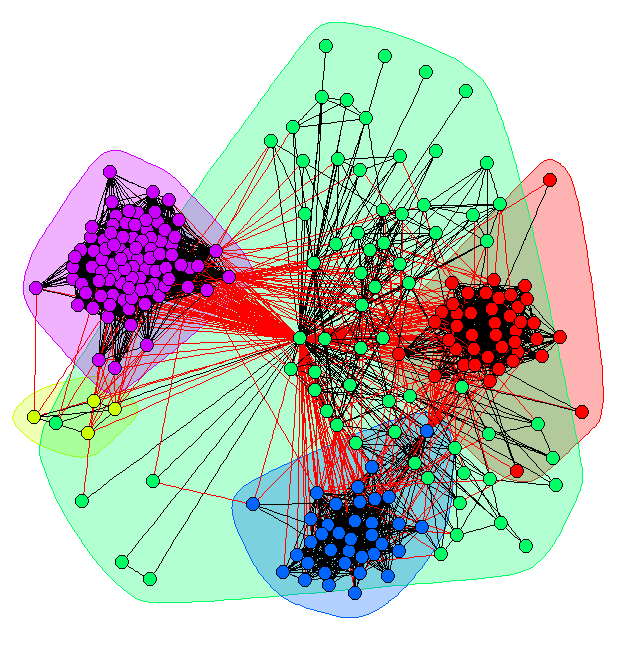
\includegraphics[width=0.7\textwidth]{social.png}
\caption{\url{http://francescopochetti.com/community-detection-social-networks/}}
\end{figure}
\end{minipage}
}

\section{Classifications of ML methods}

\frame{
\frametitle{With respect to problem formulation}
\begin{itemize}
\item Supervised learning
\item Unsupervised learning
\item Reinforcement learning
\end{itemize}
}

\frame{
\frametitle{Supervised learning}
\begin{itemize}
\item Model should establish relationship between {\em target variable} and {\em features}
\item Model allows making predictions of target variable if feature values are known
\item Input data consist of both feature values and target values
\item Term supervision refers to availability of target values
\item Task to be learned is defined by the data instead of being defined by the algorithm
\item Typical tasks:
\begin{itemize}
\item Regression
\item Classification
\end{itemize}
\end{itemize}
}

\frame{
\frametitle{Regression}
\vspace{5mm}
\begin{itemize}
\item Target variable is continuous
\item Tasks like prediction of stock prices, steering angles, resource consumption, rainfall, algorithm runtime
\end{itemize}
\vspace{-5mm}
\begin{figure}
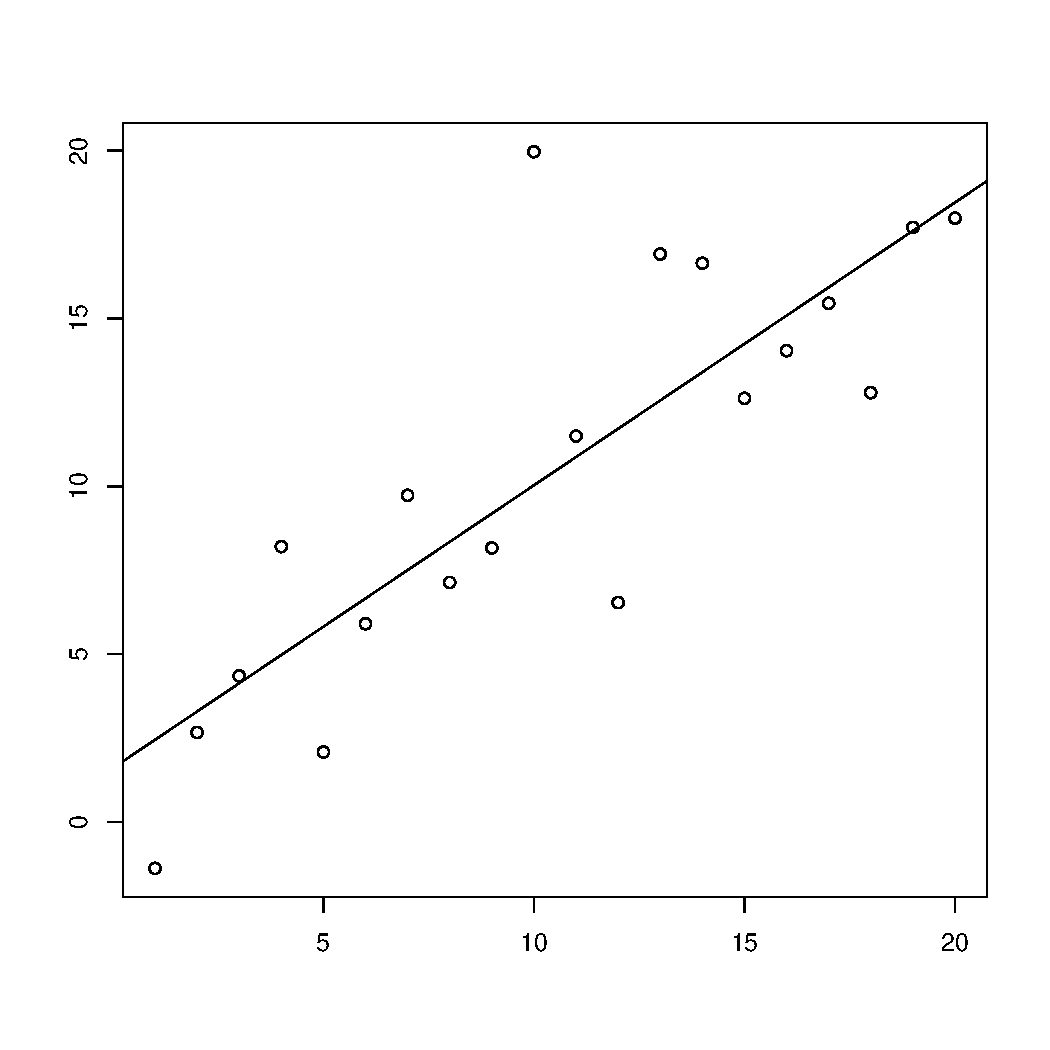
\includegraphics[width=0.35\textwidth]{reg20.pdf}
\vspace{-5mm}
\caption{P. Jani\v ci\'c, M. Nikoli\'c, Artificial intelligence, in preparation.}
\end{figure}
}

\frame{
\frametitle{Classification}
\vspace{5mm}
\begin{itemize}
\item Target variable is categorical (finite and unordered value set)
\item Tasks like face detection, object recognition, OCR, speech recognition
\end{itemize}
\begin{figure}
\resizebox{0.35\textwidth}{!}{
\input{razdvajanje.tkz}
}
\caption{P. Jani\v ci\'c, M. Nikoli\'c, Artificial intelligence, in preparation.}
\end{figure}
}


\frame{
\frametitle{Unsupervised learning}
\begin{itemize}
\item Model should identify some relevant structure in the data
\item Input data consists only of feature values, there are no target values
\item Task to be learned is defined by the algorithm -- for different kinds of tasks, different learning algorithms are formulated
\item Typical tasks:
\begin{itemize}
\item Clustering
\item Dimensionality reduction
\item Representation learning
\end{itemize}
\end{itemize}
}

\frame{
\frametitle{Clustering}
\begin{itemize}
\item Identification of groups of data
\item Grouping can be defined based on proximity, density, shape, ...
\item $k$ means, DBSCAN, Gaussian mixture, agglomerative hierarchical clustering, ...
\item Tasks like community detection in social networks, human genetic clustering, detection of different types of tissue in medical imaging, data reduction
\item Interesting both in its own right and as a data preprocessing technique
\end{itemize}
}

\frame{
\frametitle{Clustering illustration}
\begin{figure}
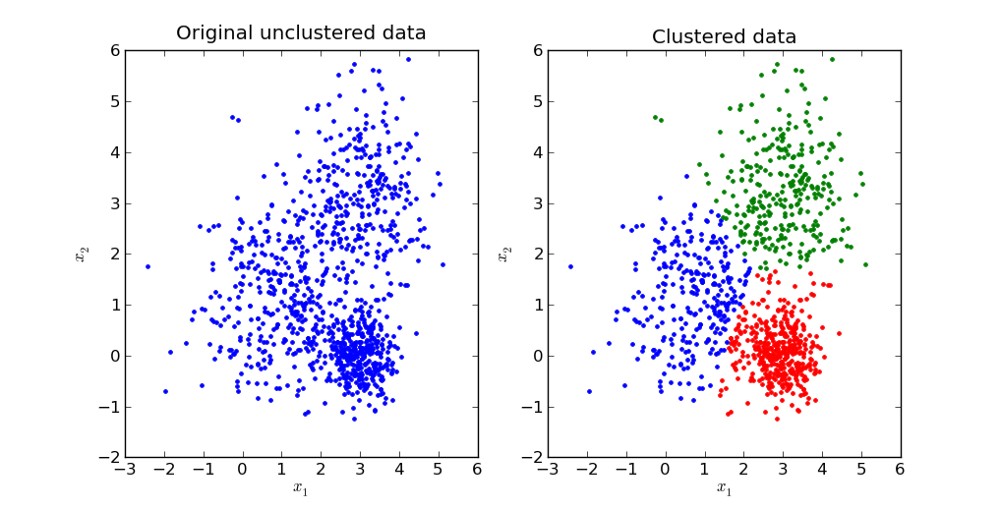
\includegraphics[width=0.8\textwidth]{clustering.png}
\vspace{-5mm}
\caption{\url{https://towardsdatascience.com/k-means-data-clustering-bce3335d2203}}
\end{figure}

}


\frame{
\frametitle{Dimensionality reduction}
\begin{itemize}
\item Identification of subspaces (planes or manifolds) in which data lie
\item PCA, autoencoders, $t$-SNE, ...
\item Mostly used for data preprocessing and visualisation
\begin{figure}
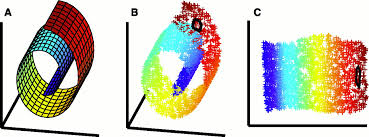
\includegraphics[width=0.8\textwidth]{ndr.jpg}
\vspace{-5mm}
\caption{S. Roweis, L. Saul, Nonlinear Dimensionality Reduction by Locally Linear Embeddings}
\end{figure}
\end{itemize}
}

\frame{
\frametitle{Representation learning}
\begin{itemize}
\item Finding representations in data which facilitate exploitation of relevant information
\item PCA, autoencoders, VAEs, GANs, word2vec,...
\item Mostly used for natural language understanding, semantic image manipulation, improvement of other algorithms...
\end{itemize}
}


\frame{
\frametitle{Reinforcement learning}
\begin{itemize}
\item Probably highest hype to utility ratio :)
\item Agent takes actions in an environment, observes its state, and receives reward from the environment for actions taken
\item Model should map states to actions, so that total obtained reward is maximal
\item Since reward is given, it is not unsupervised learning
\item Agent is not informed if the action taken in some state was the right one!!
\item Therefore it is not supervised learning, either
\item Credit assignment mechanism is needed to identify best actions based on total reward obtained
\item Control tasks in robotics, autonomous vehicle driving, therapy optimisation, dialog systems, game playing
\end{itemize}
}


\frame{
\frametitle{With respect to statistical framework}
\begin{itemize}
\item Frequentist -- most people consider it standard
\item Bayesian  -- most people consider it exotic 
\item Deep theoretical distinction, often poorly understood
\end{itemize}
}

\frame{
\frametitle{Frequentist approach}
\begin{itemize}
\item Probabilities are long term frequencies of occurrences of events
\item Stochastic behaviour of interest is determined by unknown, but fixed parameters, which are not random variables!
\item It is meaningless to talk about probabilities of parameter values, only of probabilities of events, given parameters
\item Learning consists of parameter estimation
\item Prediction consists of finding most likely values of target variable given feature values, with respect to estimated parameter values
\end{itemize}
}

\frame{
\frametitle{Bayesian approach (1)}
\begin{itemize}
\item Probabilities are degrees of belief
\item Therefore, parameters can be assigned probability distributions
\item We can have different degrees of belief about parameter values based on evidence
\item Prior convictions of parameter values are given through {\em prior distribution}, which is updated based on provided data (i.e., evidence) to yield {\em posterior distribution}
\item Learning consists of estimation of posterior distribution of parameters
\item Prediction consists of (weighted) averaging of predictions which all possible parameter values would yield according to posterior distribution, given feature values
\end{itemize}
}

\frame{
\frametitle{Bayesian approach (2)}
\begin{itemize}
\item High mathematical overhead at algorithm design time
\item High computational overhead both at learning and inference time
\item Often provide increase in predictive performance -- due to uncertainty modelling it is less prone to overfitting
\item Often can provide more information through parameter value distributions which might offer new insights
\end{itemize}
}

\frame{
\frametitle{With respect to modelling approach}
\begin{itemize}
\item Generalized linear models
\item Rule based models
\item Instance based models
\item Artificial neural networks
\item Ensemble models
\item Latent variable models
\item Probabilistic graphical models
\end{itemize}
}

\frame{
\frametitle{Generalized linear models}
\begin{minipage}{0.49\textwidth}
\begin{itemize}
\item Based on linear model of target variable
\item Computationally efficient
\item Easily interpretable
\item Often not powerful enough in terms of predictive performance
\item Often make unrealistic assumptions
\end{itemize}
\end{minipage}
\begin{minipage}{0.49\textwidth}
\begin{figure}
\begin{center}
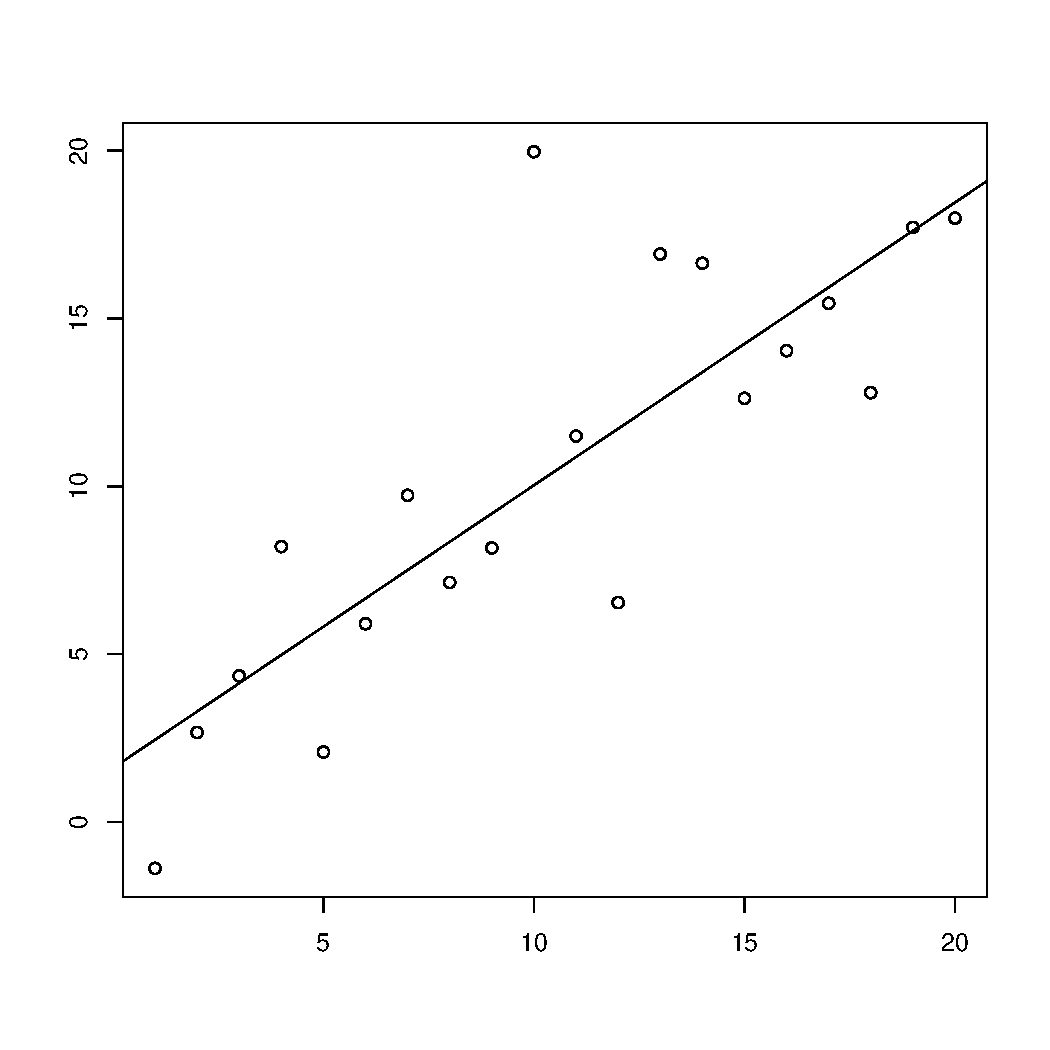
\includegraphics[width=\textwidth]{reg20.pdf}
\vspace{-5mm}
\caption{P. Jani\v ci\'c, M. Nikoli\'c, Artificial intelligence, in preparation.}
\end{center}
\end{figure}
\end{minipage}
}

\frame{
\frametitle{Rule based models}
\begin{minipage}{0.54\textwidth}
\begin{itemize}
\item Based on rules which test values of some features and make decisions based on those tests
\item Decision trees are a typical representative
\item Easily interpretable if small (but less than linear models)
\item Often more powerful than linear models
\item Still not powerful enough
\end{itemize}
\end{minipage}
\begin{minipage}{0.44\textwidth}
\begin{figure}
\begin{center}
\vspace{5mm}
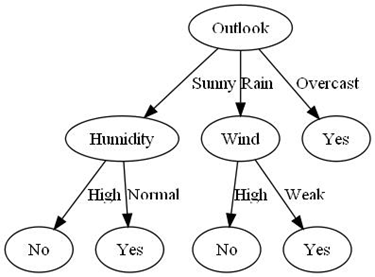
\includegraphics[width=\textwidth]{tree.png}
\caption{T. Mitchell, Machine Learning}
\end{center}
\end{figure}
\end{minipage}
}

\frame{
\frametitle{Instance based models}
\begin{minipage}{0.54\textwidth}
\begin{itemize}
\item Compare an input instance to already known examples to make inference
\item Make fewer unrealistic assumptions
\item Require memory to store existing examples
\item Can be slow in prediction time due to comparisons that are made
\item Not interpretable
\end{itemize}
\end{minipage}
\begin{minipage}{0.44\textwidth}
\begin{figure}
\begin{center}
\vspace{8mm}
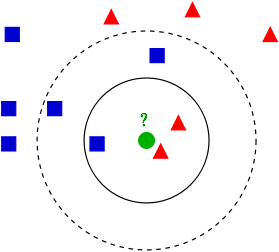
\includegraphics[width=\textwidth]{knn.png}
\vspace{-5mm}
\caption{\url{https://en.wikipedia.org/wiki/K-nearest_neighbors_algorithm}}
\end{center}
\end{figure}
\end{minipage}
}

\frame{
\frametitle{Artificial neural networks}
\begin{minipage}{0.64\textwidth}
\begin{itemize}
\item Biologically inspired models very roughly resembling functioning of biological neurons
\item Can be thought of as of composition of many generalized linear models
\item Specially suitable for processing large quantities of raw rata (text, images, video, sound)
\item Very powerful in terms of predictive performance
\item Tricky to train
\item Computationally very demanding
\item Not interpretable
\end{itemize}
\end{minipage}
\begin{minipage}{0.35\textwidth}
\begin{figure}
\begin{center}
\vspace{4mm}
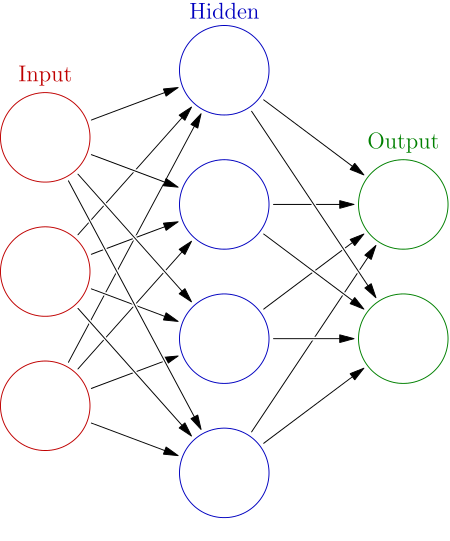
\includegraphics[width=0.9\textwidth]{ann.png}
\vspace{-5mm}
\caption{\url{https://en.wikipedia.org/wiki/Artificial_neural_network}}
\end{center}
\end{figure}
\end{minipage}
}


\frame{
\frametitle{Ensemble models}
\begin{itemize}
\item Exploit the independence of mistakes of numerous weak models to obtain good predictions by voting or averaging
\item Bagging (random decision forests), boosting (AdaBoost, gradient boosting), etc.
\item Often the best choice for vectorial data
\item Very powerful in terms of predictive performance
\item Often not hard to train
\item Can be computationally demanding, but that depends on the kind of models being combined
\item Not interpretable
\end{itemize}
}

\frame{
\frametitle{Probabilistic graphical models}
\begin{itemize}
\item Model dependencies between multiple target variables, not only between a target variable and features
\item Sometimes features do not explain behaviour of target variables, but correlations between them can be observed and exploited
\item Provide confidence information (dependent on the chosen probabilistic model)
\item Mathematically challenging
\item High computation cost, even in prediction time!
\item Tasks like social network analysis, image segmentation, pixel classification, natural language processing, environmental data modelling
\end{itemize}
}

\section{Supervised ML Fundamentals}

\frame{
\frametitle{Loss and risk}
\begin{itemize}
\item There is a relationship between $x$ and $y$
\item We are aware of that relationship via sample ${\cal D}=\{(x_i,y_i)\ |\ i=1,\ldots, N\}$
\item Find ''the best`` function $f$ such that $y\approx f(x)$
\item Let {\em loss function} $L$ quantify the discrepancy between $y$ and $f(x)$
\item Loss is averaged over the training set to obtain {\em error function} or {\em empirical risk}
$$E(f,{\cal D})=\frac{1}{N}\sum_{i=1}^NL(y_i,f(x_i))$$
\item {\em Emprirical risk minimization principle}: find the model which minimizes $E$
\end{itemize}
}

\frame{
\frametitle{Model representation}
\begin{itemize}
\item Considering all possible models is infeasible, so a {\em model representation} is assumed
\item We assume that the model $f_w(x)$ is determined by a set of {\em model parameters} $w$, so the error function can be written $E(w,{\cal D})$
\end{itemize}
}


\frame{
\frametitle{ERM for classification}
\begin{itemize}
\item What should we minimize?
\item<2> Minimize the number of training errors
\item<2> Indicator function:
$$I(F)=\left\{\begin{array}{ll}1 & \text{if } F\\0 & \text{if }\neg F\end{array}\right.$$
\item<2> Loss: $L(u,v)=I(u\neq v)$
\item<2> Optimization problem:
$$\min_{w}\frac{1}{N}\sum_{i=1}^NI(y_i\neq f_w(x_i))$$
\end{itemize}
}

\frame{
\frametitle{Regression}
\vspace{6mm}
\begin{figure}
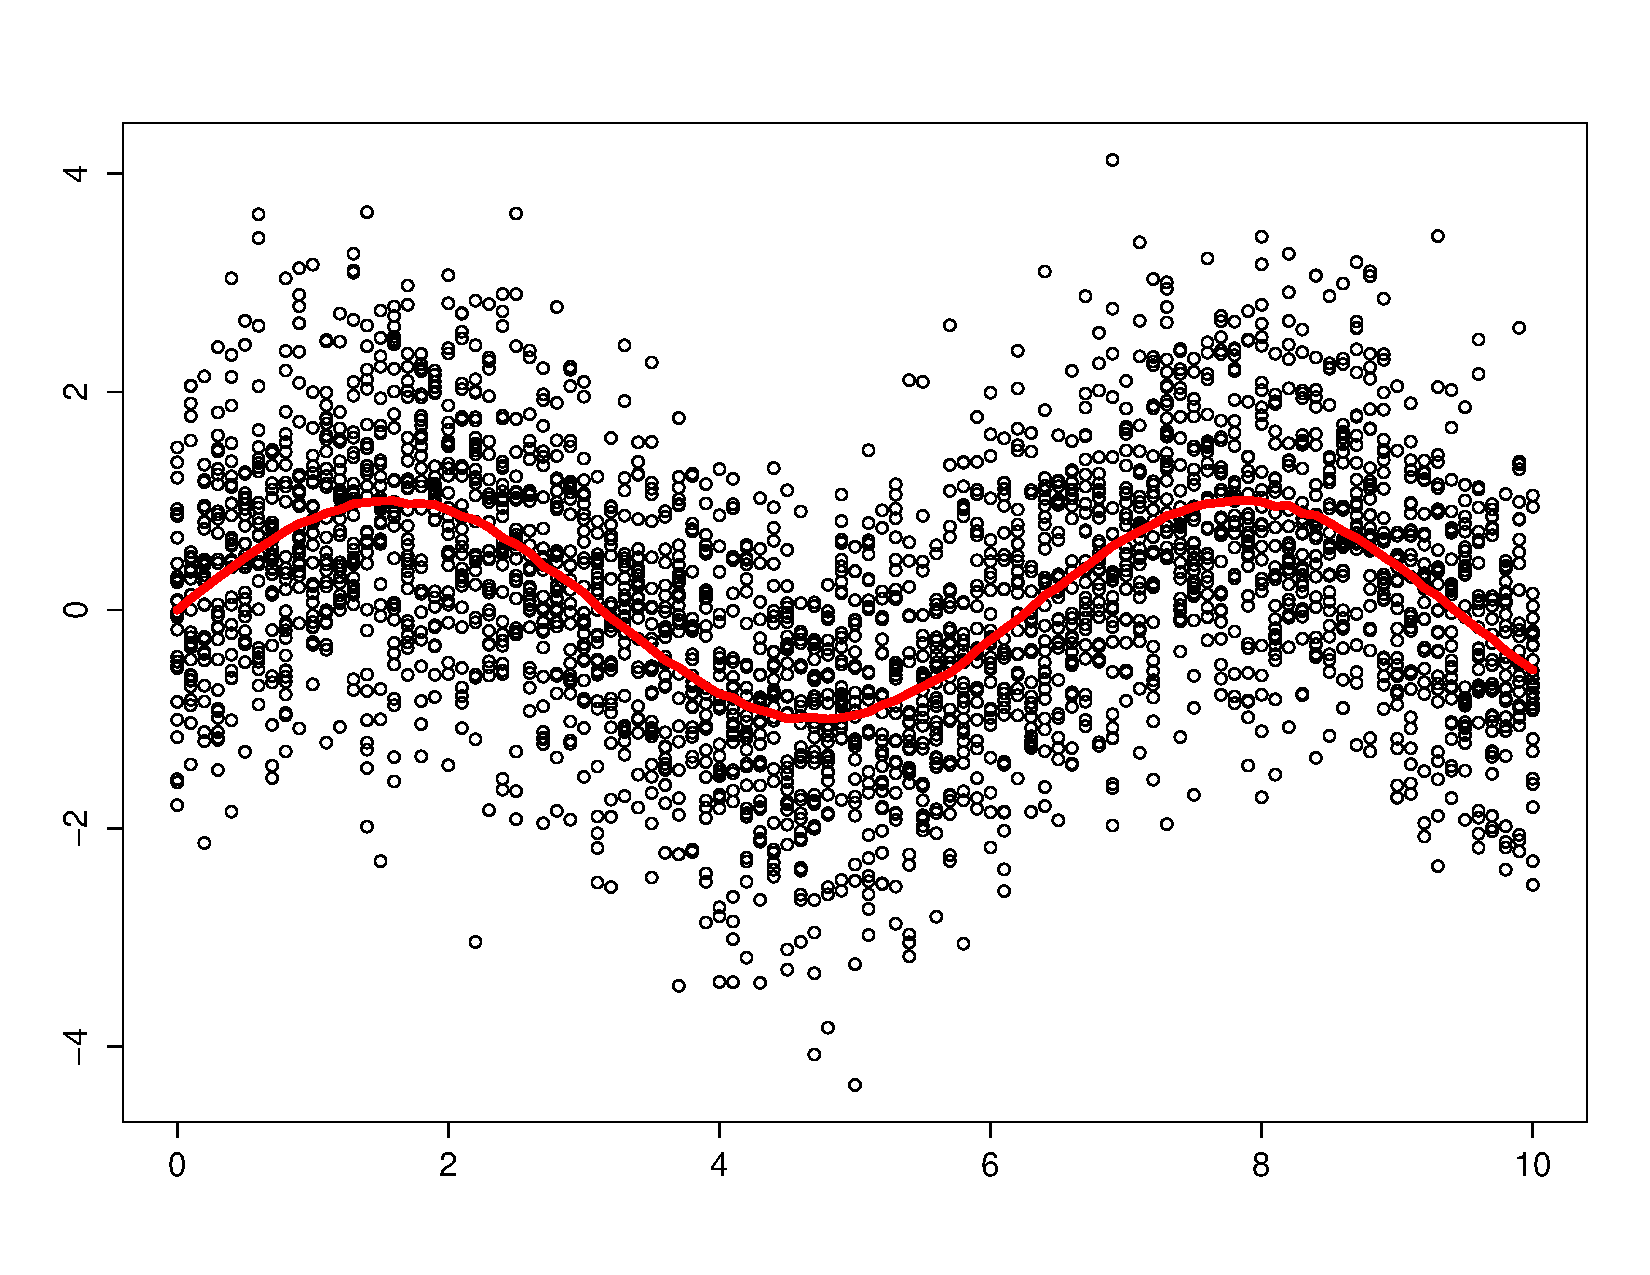
\includegraphics[width=0.555\textwidth]{reg.pdf}
\caption{P. Jani\v ci\'c, M. Nikoli\'c, Artificial intelligence, in preparation.}
\end{figure}
}

\frame{
\frametitle{Regression}
\begin{itemize}
\item Regression function: $r(x)=\mathbb{E}(y|x)=\int y\ p(y|x)dy$
\item If $r(x)=f_w(x)$ for some $w$, then it is a minimizer of
$$\mathbb{E}[(y-f_w(x))^2]$$
\item In general, the minimum is attained for the function closest\footnote{\hspace{1cm}With respect to $\ell_2$ norm} to $r(x)$
\end{itemize}
}

\frame{
\frametitle{ERM for regression}
\begin{itemize}
\item Loss:
$$L(u,v)=(u-v)^2$$
\item Optimization problem:
$$\min_{w}\frac{1}{N}\sum_{i=1}^N(y_i-f_w(x_i))^2$$
\end{itemize}
}

\frame{
\frametitle{How well can we fit a model?}
\begin{itemize}
\item Consider regression problem
\item Simple linear regression: $f_w(x)=w_0+w_1 x$
\item Polynomial linear regression: $f_w(x)=\sum_{i=0}^n w_i x^i$
\end{itemize}
}

\frame{
\frametitle{Simple linear regression}
\vspace{-0.3cm}
\begin{figure}
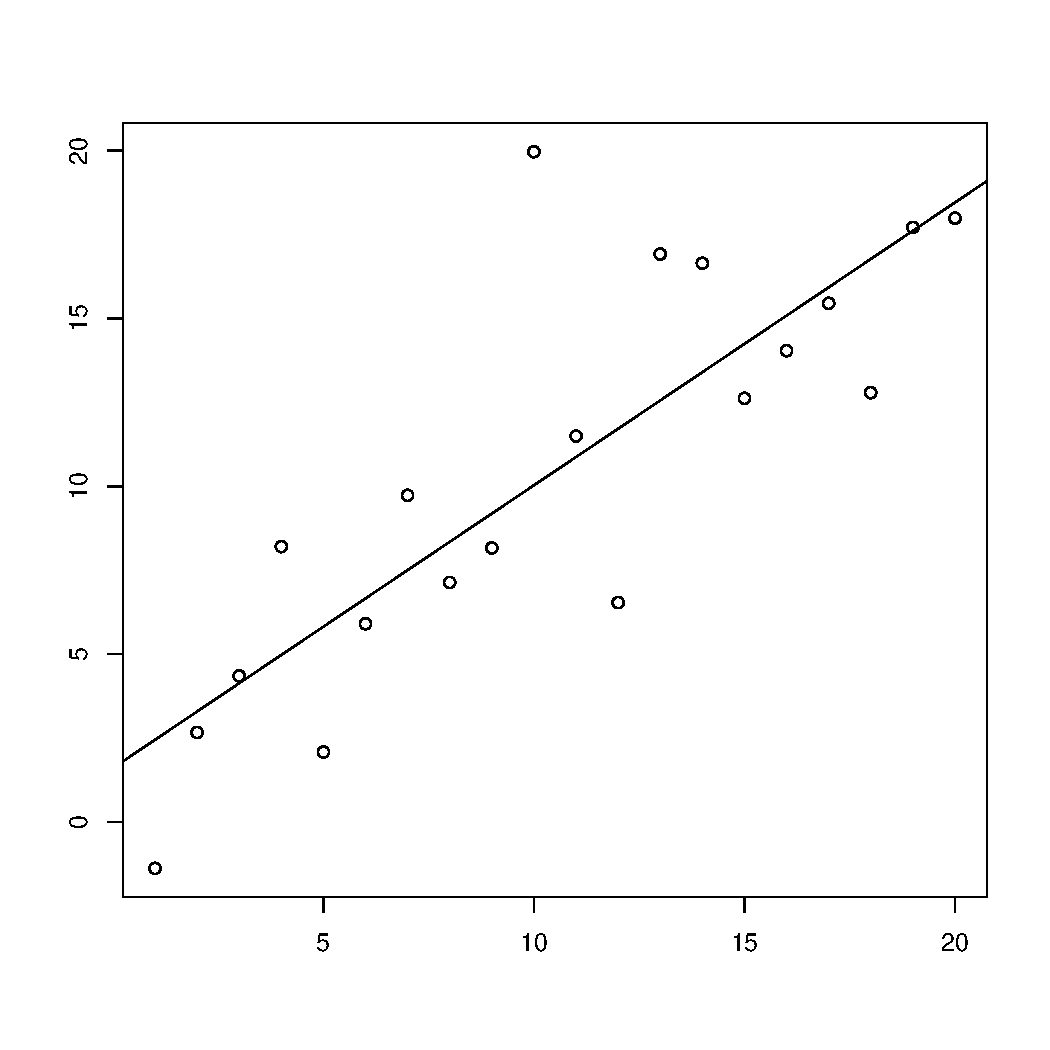
\includegraphics[width=0.55\textwidth]{reg20.pdf}
\vspace{-7.9mm}
\caption{P. Jani\v ci\'c, M. Nikoli\'c, Artificial intelligence, in preparation.}
\end{figure}
}

\frame{
\frametitle{Polynomial linear regression}
\vspace{-0.3cm}
\begin{figure}
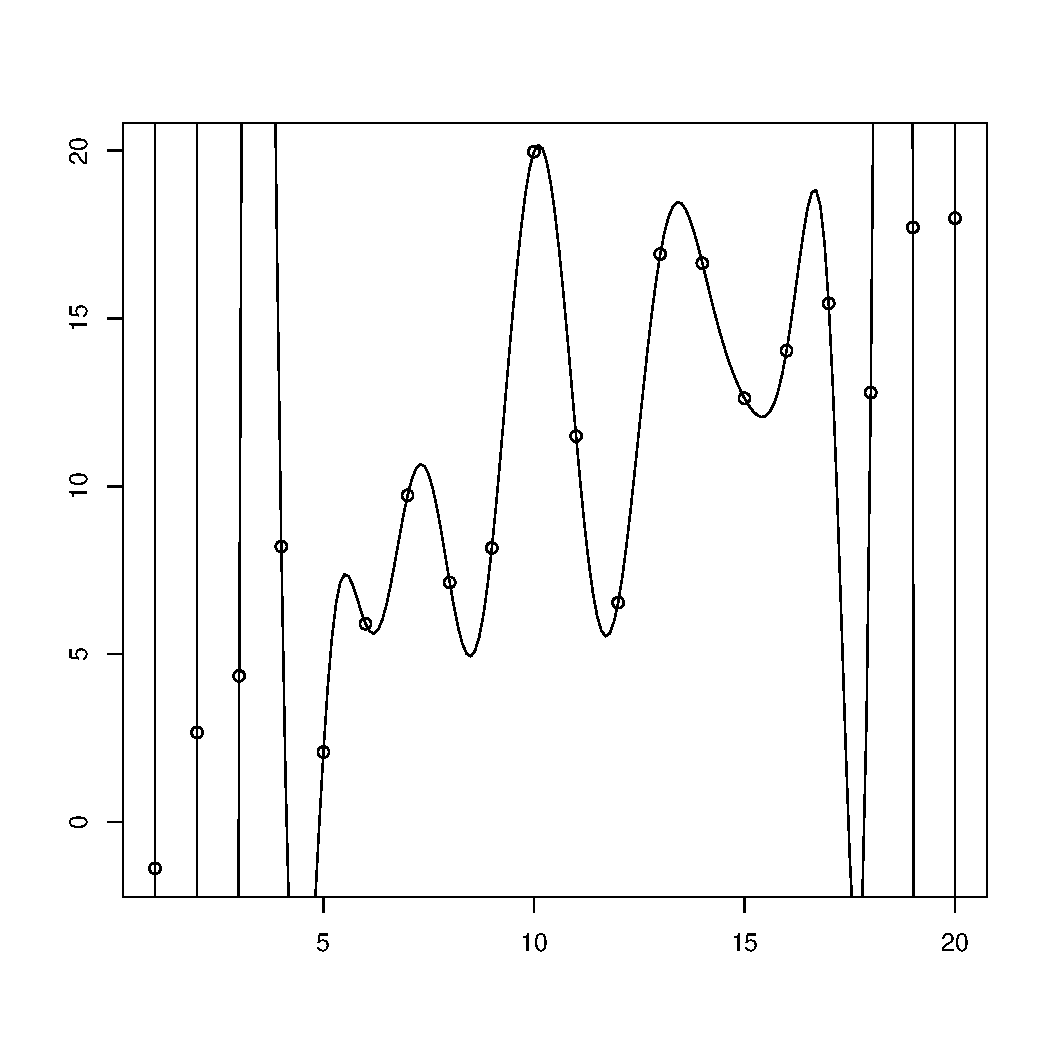
\includegraphics[width=0.55\textwidth]{interpolacija.pdf}
\vspace{-7.9mm}
\caption{P. Jani\v ci\'c, M. Nikoli\'c, Artificial intelligence, in preparation.}
\end{figure}
}

\frame{
\frametitle{Overfitting}
\begin{itemize}
\item Good fit of the model on the training data does not mean good generalization
\item Compare to rote learning
\item Caused by model flexibility (often called complexity)
\item Controlling model flexibility is of paramount importance for good generalization
\item One of central topics of machine learning and source of it's deepest theory
\end{itemize}
}

\frame{
\frametitle{How to make models less flexible?}
\begin{itemize}
\item Restrict model representation (e.g. linear models)?
\item<2-3> Possible, but that approach may be too rigid
\item<3> Given a very flexible model representation, can flexibility be tuned based on model's performance?
\end{itemize}
}


\frame{
\frametitle{Regularization (1)}
\begin{itemize}
\vspace{-2mm}
\item Minimization of regularized empirical risk:
$$\min_{w}\frac{1}{N}\sum_{i=1}^NL(y_i,f_w(x_i))+\lambda\Omega(w)$$
\item Frequent choice of {\em regularization term} is squared $\ell_2$ norm
$$\Omega(w)=\|w\|^2_2=\sum_{i=1}^nw_i^2$$
\item Regularization term penalizes the magnitude of the parameters, making the model less adaptable to the data
\item {\em Regularization meta-parameter} $\lambda$ tunes model flexibility/complexity
\end{itemize}
}

\frame{
\frametitle{Regularization (2)}
\begin{itemize}
\item In case of linear models, it holds $$\|w\|_2=\|\nabla_x f_w(x)\|_2$$
\item Constraining the gradient makes function more smooth
\item In a more general sense, regularization is any modification of optimization problem that restricts model flexibility and makes it less susceptible to overfitting
\item In an even more general sense, regularization is any modification of a mathematical problem which makes it less sensitive to changes in input parameters
\end{itemize}
}

\frame{
\frametitle{Regularization example -- classification models}
\begin{itemize}
\item Linear classification model:
$$f_w(x)=w_0+w_1x_1+w_2x_2$$
\item Polynomial classification model:
$$f_w(x)=\sum_{i=1}^n\sum_{j=0}^iw_{ij}x_1^jx_2^{i-j}$$
\end{itemize}
}

\frame{
\frametitle{Regularization example -- data points}
\vspace{6mm}
\begin{figure}
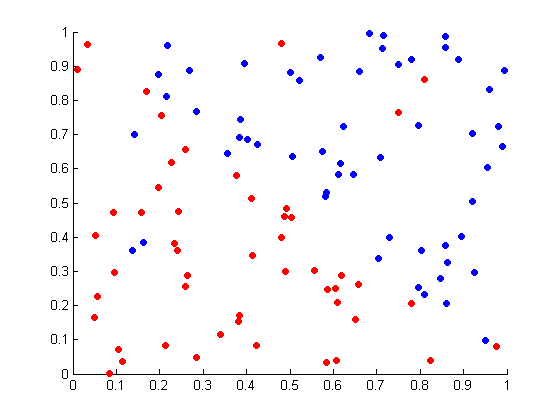
\includegraphics[width=0.57\textwidth]{tacke.png}
\vspace{0.02cm}
\caption{P. Jani\v ci\'c, M. Nikoli\'c, Artificial intelligence, in preparation.}
\end{figure}
}

\frame{
\frametitle{Regularization example -- linear classifier prediction}
\begin{adjustwidth}{-1.4cm}{0cm}
\begin{figure}
\vspace{2mm}
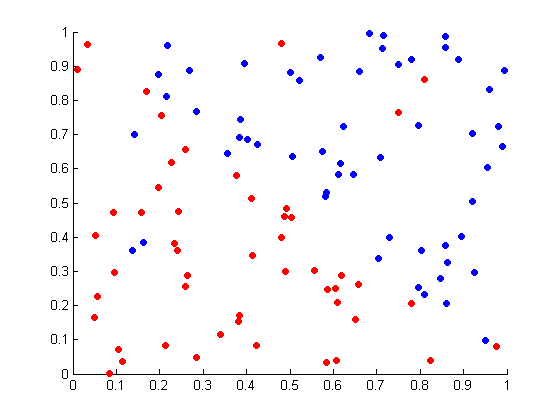
\includegraphics[width=0.59\textwidth]{tacke.png}
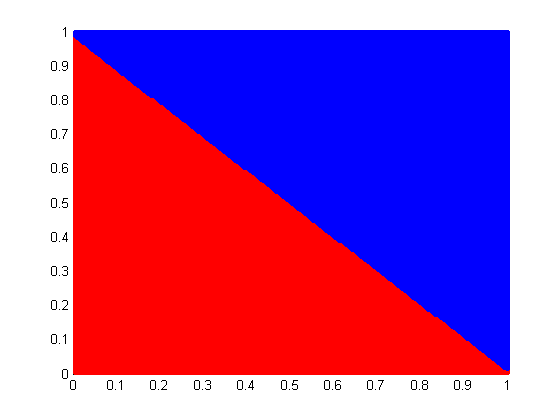
\includegraphics[width=0.59\textwidth]{linear.png}
\vspace{-1.3mm}
\caption{P. Jani\v ci\'c, M. Nikoli\'c, Artificial intelligence, in preparation.}
\end{figure}
\end{adjustwidth}
}

\frame{
\frametitle{Regularization example -- polynomial classifier prediction}
\begin{adjustwidth}{-1.4cm}{0cm}
\begin{figure}
\vspace{2mm}
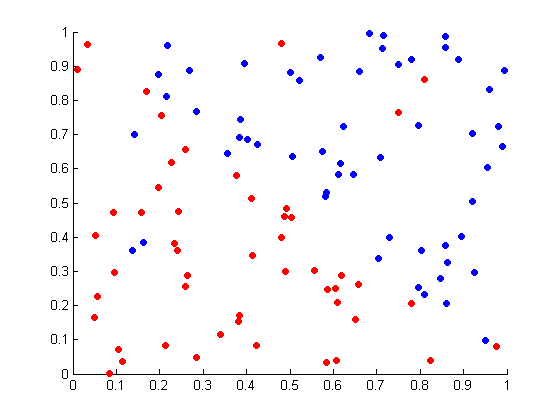
\includegraphics[width=0.59\textwidth]{tacke.png}
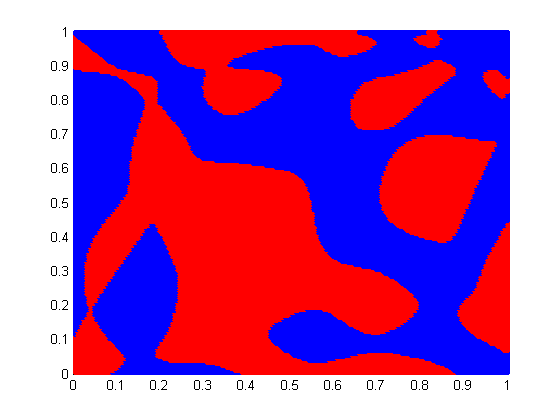
\includegraphics[width=0.59\textwidth]{polinom.png}
\vspace{-1.3mm}
\caption{P. Jani\v ci\'c, M. Nikoli\'c, Artificial intelligence, in preparation.}
\end{figure}
\end{adjustwidth}
}


\frame{
\frametitle{Regularization example -- regularized poly. prediction}
\begin{adjustwidth}{-1.4cm}{0cm}
\begin{figure}
\vspace{2mm}
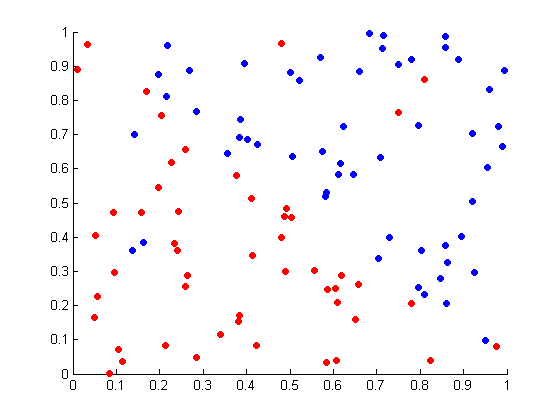
\includegraphics[width=0.59\textwidth]{tacke.png}
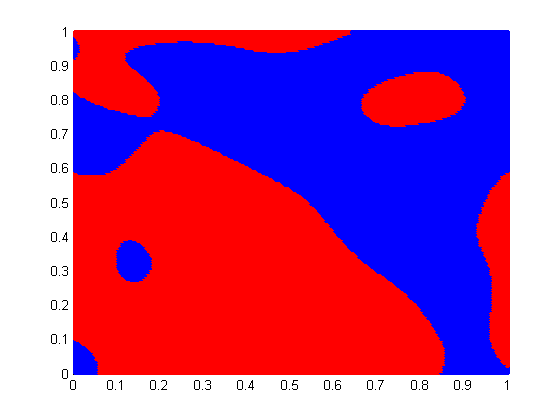
\includegraphics[width=0.59\textwidth]{10-9.png}
\vspace{-1.3mm}
\caption{P. Jani\v ci\'c, M. Nikoli\'c, Artificial intelligence, in preparation.}
\end{figure}
\end{adjustwidth}
}

\frame{
\frametitle{Regularization example -- regularized poly. prediction}
\begin{adjustwidth}{-1.4cm}{0cm}
\begin{figure}
\vspace{2mm}
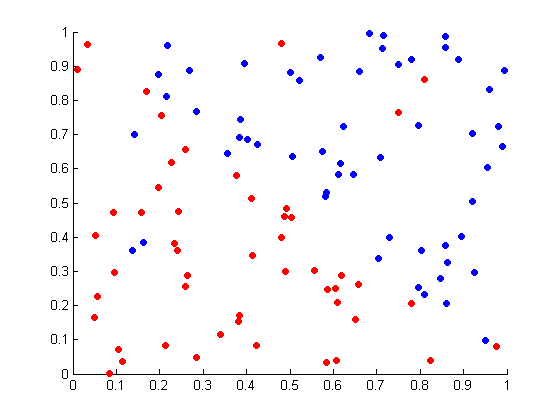
\includegraphics[width=0.59\textwidth]{tacke.png}
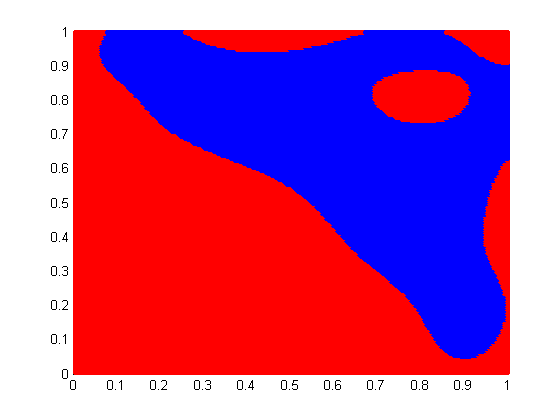
\includegraphics[width=0.59\textwidth]{10-6.png}
\vspace{-1.3mm}
\caption{P. Jani\v ci\'c, M. Nikoli\'c, Artificial intelligence, in preparation.}
\end{figure}
\end{adjustwidth}
}

\frame{
\frametitle{Regularization example -- regularized poly. prediction}
\begin{adjustwidth}{-1.4cm}{0cm}
\begin{figure}
\vspace{2mm}
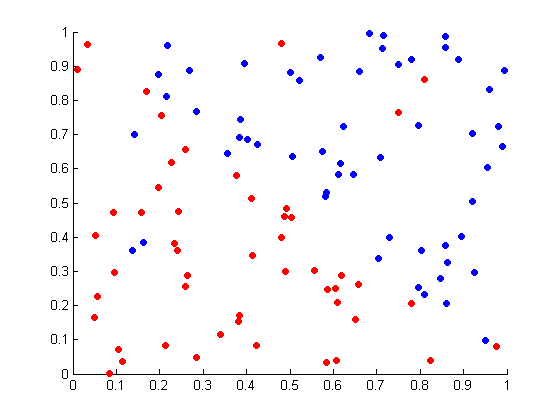
\includegraphics[width=0.59\textwidth]{tacke.png}
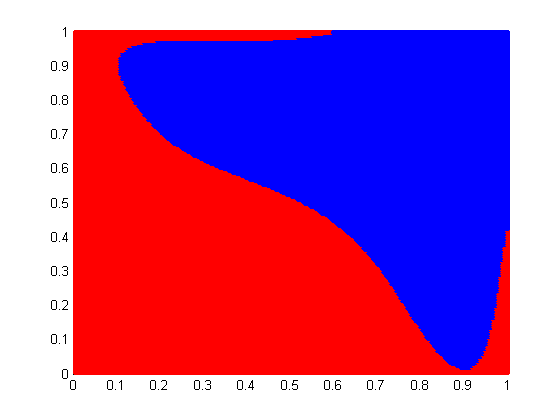
\includegraphics[width=0.59\textwidth]{10-3.png}
\vspace{-1.3mm}
\caption{P. Jani\v ci\'c, M. Nikoli\'c, Artificial intelligence, in preparation.}
\end{figure}
\end{adjustwidth}
}


\frame{
\frametitle{Regularization example -- regularized poly. prediction}
\begin{adjustwidth}{-1.4cm}{0cm}
\begin{figure}
\vspace{2mm}
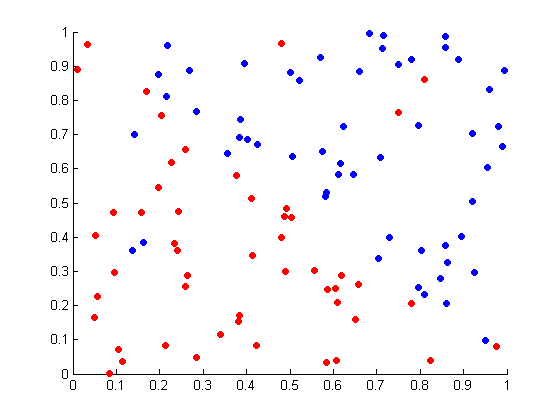
\includegraphics[width=0.59\textwidth]{tacke.png}
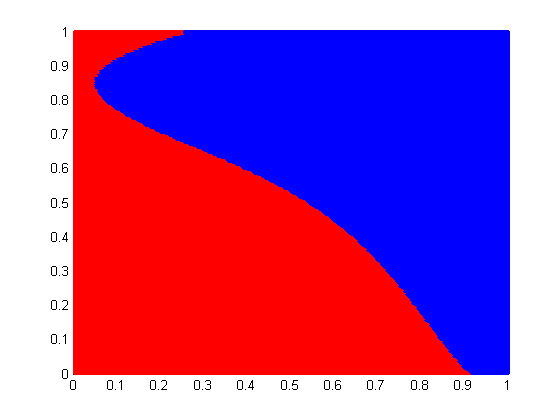
\includegraphics[width=0.59\textwidth]{10-0.png}
\vspace{-1.3mm}
\caption{P. Jani\v ci\'c, M. Nikoli\'c, Artificial intelligence, in preparation.}
\end{figure}
\end{adjustwidth}
}

\frame{
\frametitle{Regularization example -- regularized poly. prediction}
\begin{adjustwidth}{-1.4cm}{0cm}
\begin{figure}
\vspace{2mm}
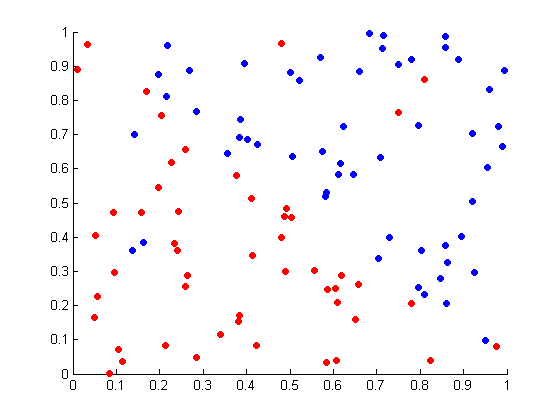
\includegraphics[width=0.59\textwidth]{tacke.png}
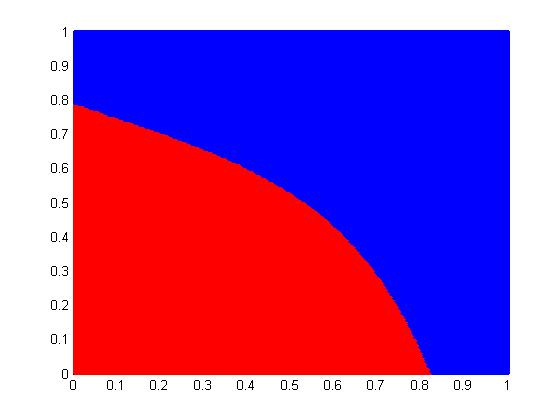
\includegraphics[width=0.59\textwidth]{10+1.png}
\vspace{-1.3mm}
\caption{P. Jani\v ci\'c, M. Nikoli\'c, Artificial intelligence, in preparation.}
\end{figure}
\end{adjustwidth}
}

\frame{
\frametitle{Regularization example -- regularized poly. prediction}
\begin{adjustwidth}{-1.4cm}{0cm}
\begin{figure}
\vspace{2mm}
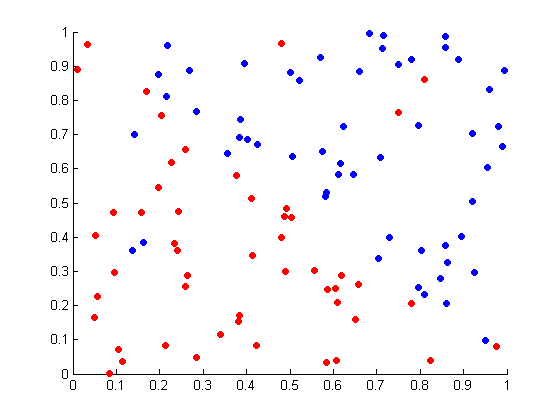
\includegraphics[width=0.59\textwidth]{tacke.png}
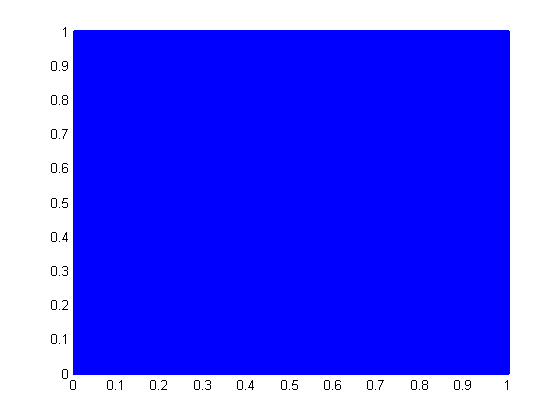
\includegraphics[width=0.59\textwidth]{10+2.png}
\vspace{-1.3mm}
\caption{P. Jani\v ci\'c, M. Nikoli\'c, Artificial intelligence, in preparation.}
\end{figure}
\end{adjustwidth}
}

\frame{
\frametitle{How to minimize error function?}
\begin{itemize}
\item Anlytically by setting gradients to zero. Often impossible.
\item Numerically by iteratively moving towards lower values of the function.
\item What is the direction of steepest descent?
\item Differentiable error functions allow for use of gradients (direction of steepest ascent)
\item Cautious move in opposite direction leads to decrease of error function value
\end{itemize}
}

\frame{
\frametitle{Gradient}
\begin{figure}
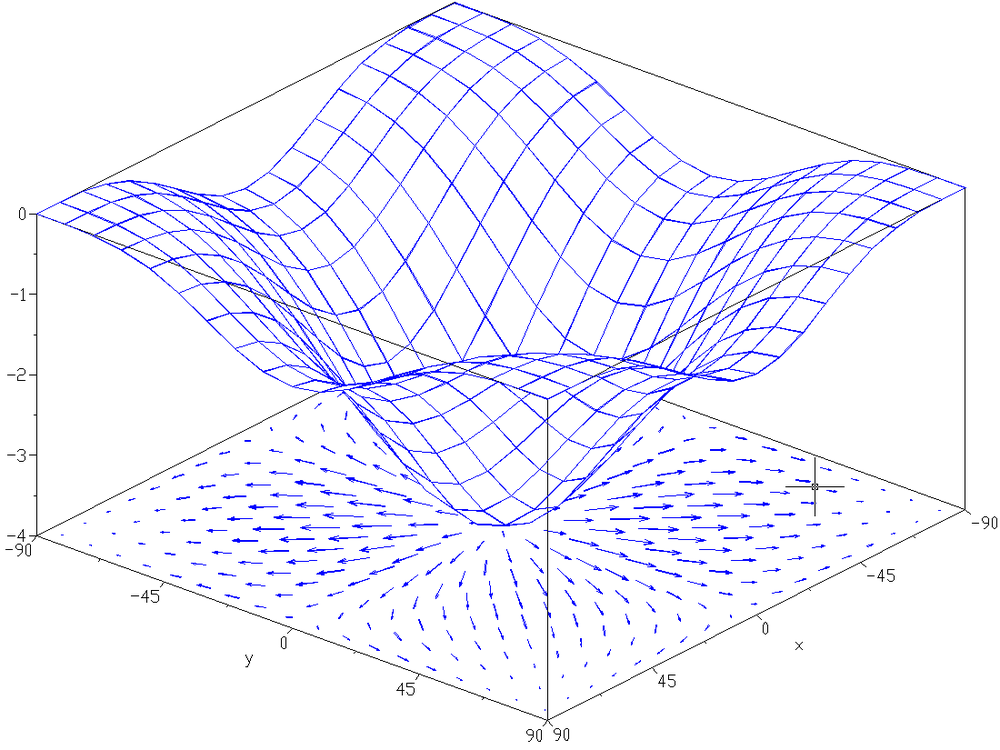
\includegraphics[width=0.55\textwidth]{gradient.png}
\vspace{-0.2cm}
\caption{math.wikia.com/wiki/Gradient}
\end{figure}
}

\frame{
\frametitle{Gradient descent}
\begin{itemize}
\item Repeat until convergence:
$$w_{k+1}=w_k-\mu_k\nabla E(w_k,{\cal D})$$
\item How to select step size $\mu_k$?
\item Fixed step size is often used, but there are better choices
\end{itemize}
}

\frame{
\frametitle{Gradient descent}
\vspace{6mm}
\begin{figure}
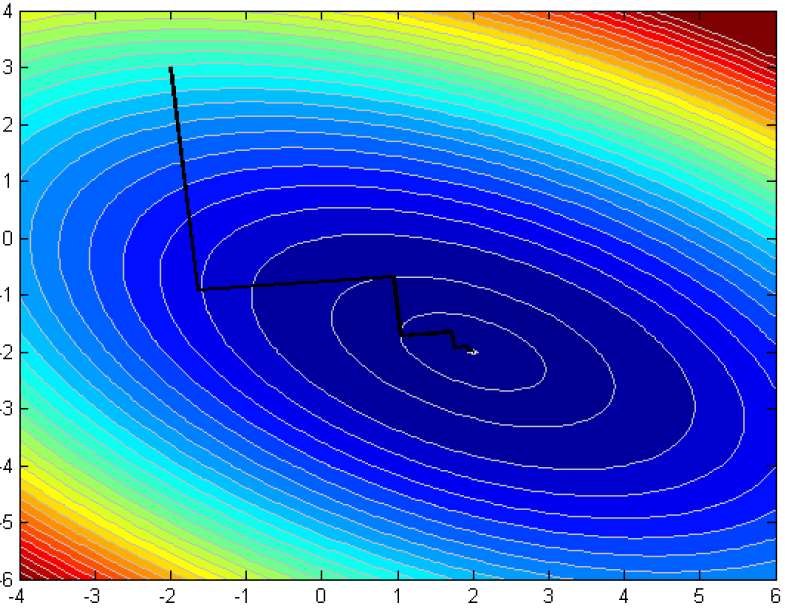
\includegraphics[width=0.57\textwidth]{graddesc.png}
\vspace{-2mm}
\caption{Y. Li, Course materials.}
\end{figure}
}


\section{Linear regression}

\frame{
\frametitle{Model}
\begin{itemize}
\item Assume linear model:
$$f_w(x)=w_0+\sum_{i=1}^{n}w_ix_i$$
\item Let's go probabilistic!
$$p_w(y|x)={\cal N}(w\cdot x,\sigma^2)$$
\end{itemize}
}

\frame{
\frametitle{Illustration}
\vspace{6mm}
\begin{figure}
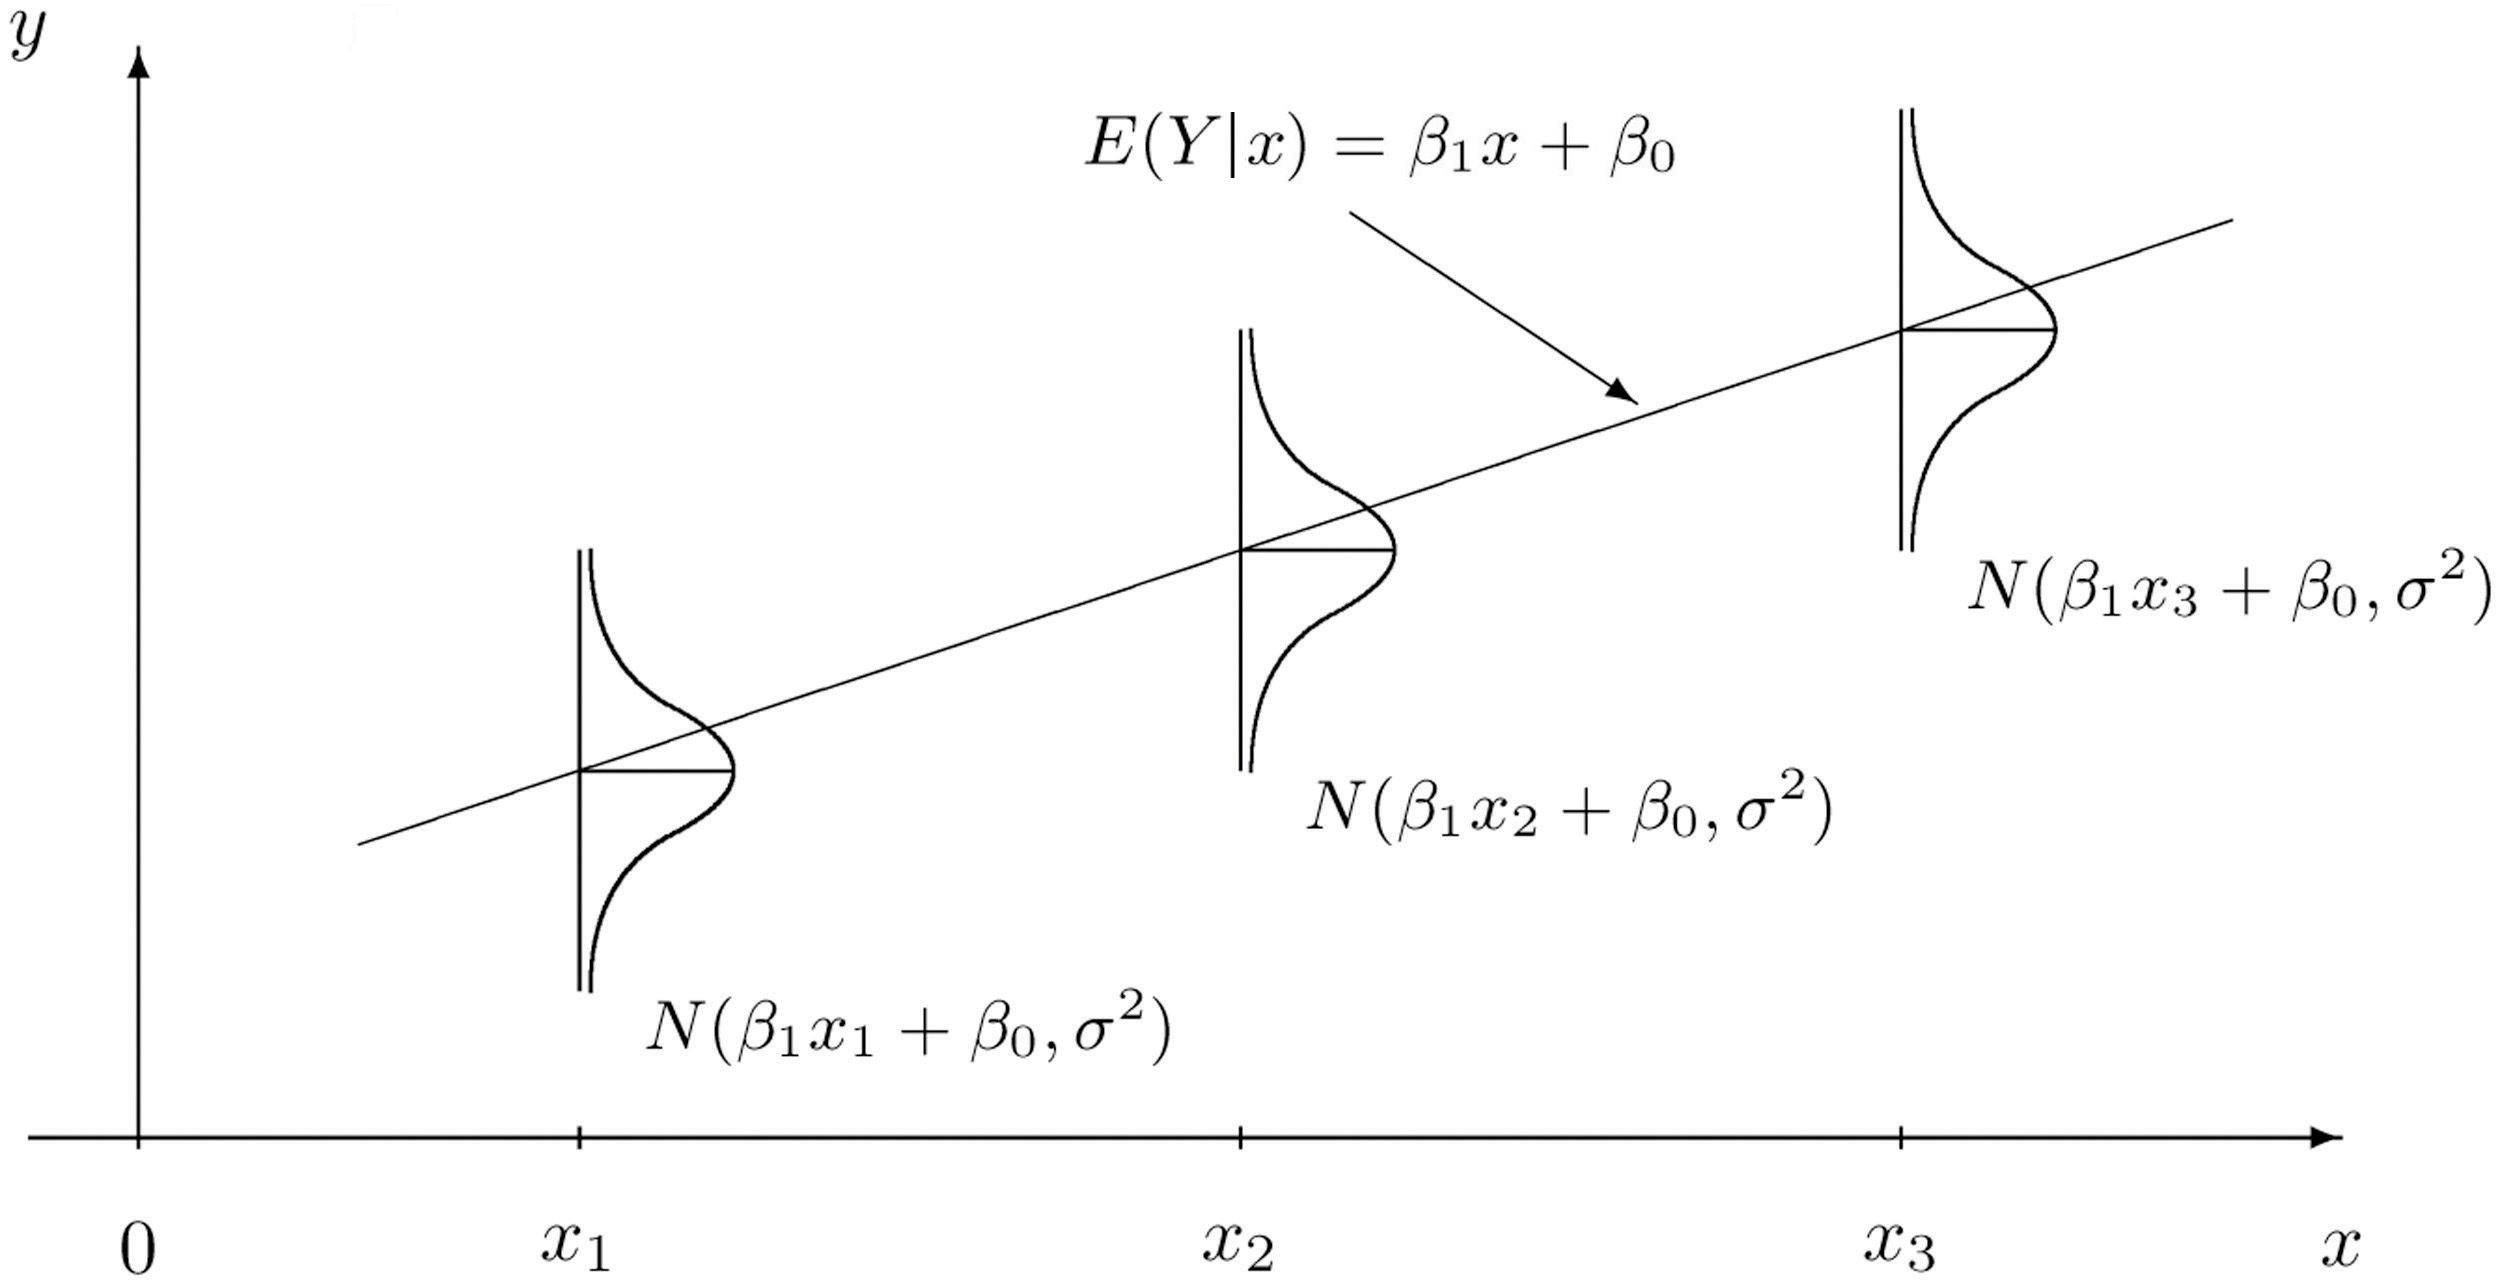
\includegraphics[width=0.835\textwidth]{linreg.jpg}
\caption{D. Shafer, Z. Zhang, Introductory Statistics, 2012.}
\end{figure}
}

\frame{
\frametitle{Maximal likelihood principle (1)}
\begin{itemize}
\item How to choose $w$?
\item Probability of observing the training set is (assuming IID)
$$\prod_{i=1}^N p_w(y_i|x_i)$$
where
$$p_w(y|x)=\frac{1}{\sqrt{2\pi\sigma^2}}\exp\left(-\frac{(y-w\cdot x)^2}{2\sigma^2}\right)$$
\item As a function of $w$ it is called {\em likelihood}
\item We are interested in {\em maximal likelihood estimate} of the parameters -- the parameter values under which the data is most likely
\end{itemize}
}

\frame{
\frametitle{Maximal likelihood principle (2)}
\begin{itemize}
\item It is more suitable to minimize negative $\log$ likelihood of the parameters:
$$NLL(w)=-\log\prod_{i=1}^N\frac{1}{\sqrt{2\pi\sigma^2}}\exp\left(-\frac{(y_i-w\cdot x_i)^2}{2\sigma^2}\right)$$
$$NLL(w)=\frac{N}{2}\log 2\pi+N\log\sigma+\frac{1}{2\sigma^2}\sum_{i=1}^N(y_i-w\cdot x_i)^2$$
\item Learning problem:
$$\min_w\sum_{i=1}^N(y_i-w\cdot x_i)^2$$
\end{itemize}
}


\frame{
\frametitle{Solution (1)}
\begin{itemize}
\item Matrix formulation
$$\min_w\|y-Xw\|^2_2$$
\item It is a convex problem!
\item Ideally $$Xw=y$$
so, ideally, $$w=X^{-1}y$$
but, in general, $X$ is not quadratic, nor invertible
\item Let's set derivatives of error function to 0
\end{itemize}
$$E(w)=\|y-Xw\|^2=(y-Xw)^T(y-Xw)$$
$$\nabla E(w)=2X^T(y-Xw)=0$$
$$w=(X^TX)^{-1}X^Ty$$
}

\frame{
\frametitle{Solution (2)}
\begin{itemize}
\item Interestingly $(X^TX)^{-1}X^T$ behaves like one would expect nonexistent $X^{-1}$ to behave:
$$\underbrace{(X^TX)^{-1}X^T}_{\text{pseudoinverse}}X=I$$
\item If the matrices are too big for inversion or even storing in memory, gradient based methods can be used
\end{itemize}
}

\frame{
\frametitle{Interpretability}
\begin{itemize}
\item Magnitude of parameters reflects their relative importance \textcolor{red}{(if the features vary in the same range)}
\item Sign of a parameter reflects the direction of correlation of the corresponding feature and the target variable
\item For example, model $y=2x_1-0.1x_2+3$ suggests that feature $x_1$ affects $y$ much more strongly than feature $x_2$ and that $x_1$ affects it positively and $x_2$ negatively
\end{itemize}
}


\frame{
\frametitle{What about polynomials?}
\begin{itemize}
\item Linearity means linearity in parameters, not in features!!
\item This is a linear model: $$f_w(x)=w_0+\sum_{i=1}^n w_i x^i$$
\item It does not seem linear in coordinate system $(x)$, but it clearly is in coordinate system
$(1,x,x^2,\ldots,x^n)$
\end{itemize}
}

\frame{
\frametitle{Illustration}
\vspace{-0.3cm}
\begin{figure}
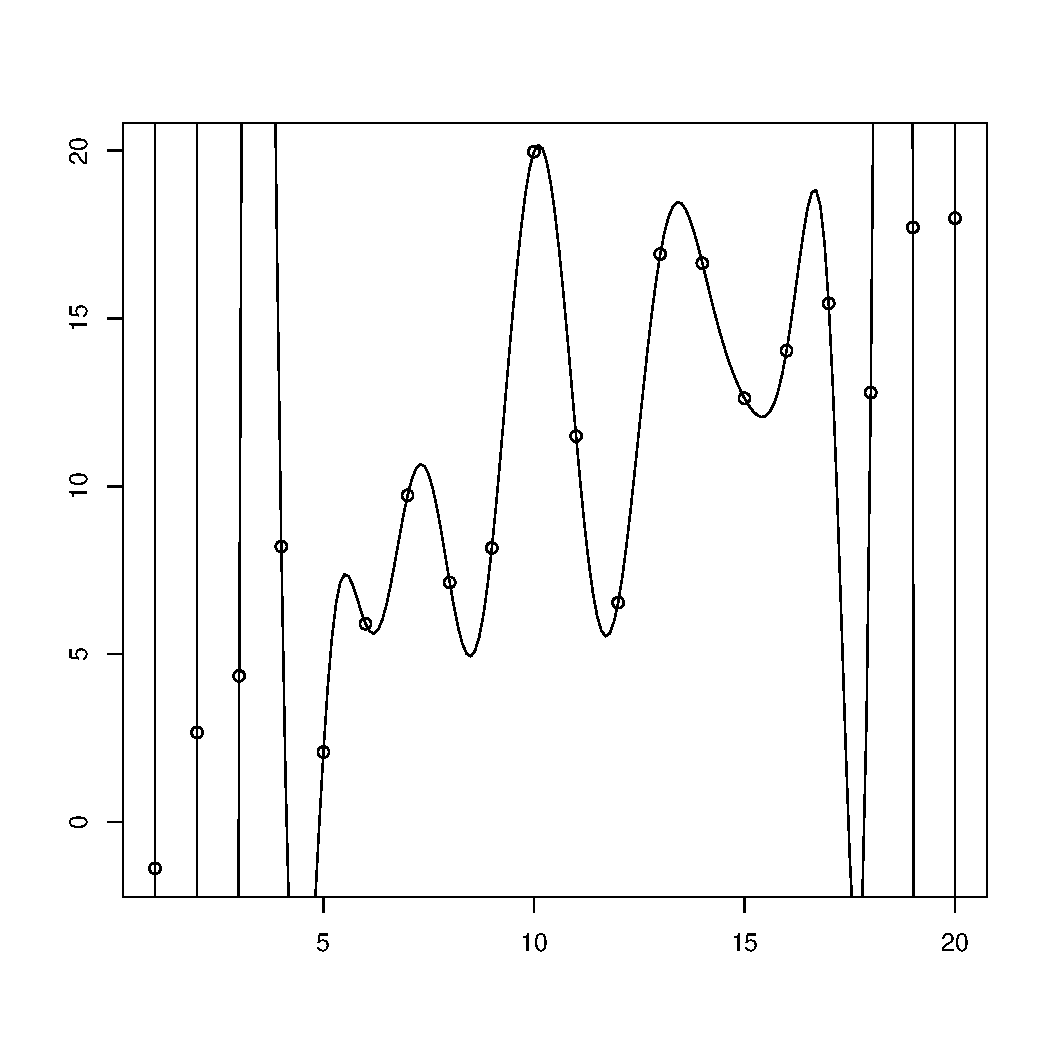
\includegraphics[width=0.55\textwidth]{interpolacija.pdf}
\vspace{-7.5mm}
\caption{P. Jani\v ci\'c, M. Nikoli\'c, Artificial intelligence, in preparation.}
\end{figure}
}

\frame{
\frametitle{Interactions}
\begin{itemize}
\item Linear model expresses independent contributions of features to target variable, which is not realistic
\item One solution is to include interactions (products of features):
$$f_w(x)=w_0+\sum_{i=1}^n w_i x_i+\sum_{i=1}^n\sum_{j=i}^n w_{ij} x_ix_j$$
\item The model is still linear, but the contribution of $x_i$ can be dependent on $x_j$ if it benefits the prediction
\end{itemize}
}

\frame{
\frametitle{Ridge regression}
\begin{itemize}
\item If the features are linearly dependent, matrix $X^TX$ is not invertible
\item If they are highly correlated, it is ill-conditioned
\item Therefore, regularized problem is considered
$$\min_w\sum_{i=1}^N(y_i-w\cdot x_i)^2+\lambda \|w\|_2^2$$
\item The solution
$$w=(X^TX+\lambda I)^{-1}X^Ty$$
\item Adding $\lambda I$ makes it a full rank matrix
\end{itemize}
}


\section{Logistic regression}
\frame{
\frametitle{Going binary}
\begin{itemize}
\item Assume classification task and let $y\in\{0,1\}$
\item Linear model approximates values $\{0,1\}$ very badly:
$$f_w(x)=w_0+\sum_{i=1}^{n}w_ix_i$$
\item But it can be squashed to the interval $(0,1)$ using {\em sigmoid function}:
$$\sigma(x)=\frac{1}{1+\exp(-x)}$$
\item The model:
$$f_w(x)=\sigma(w\cdot x)$$
\end{itemize}
}

\frame{
\frametitle{Sigmoid function}
\begin{figure}
\vspace{-2mm}
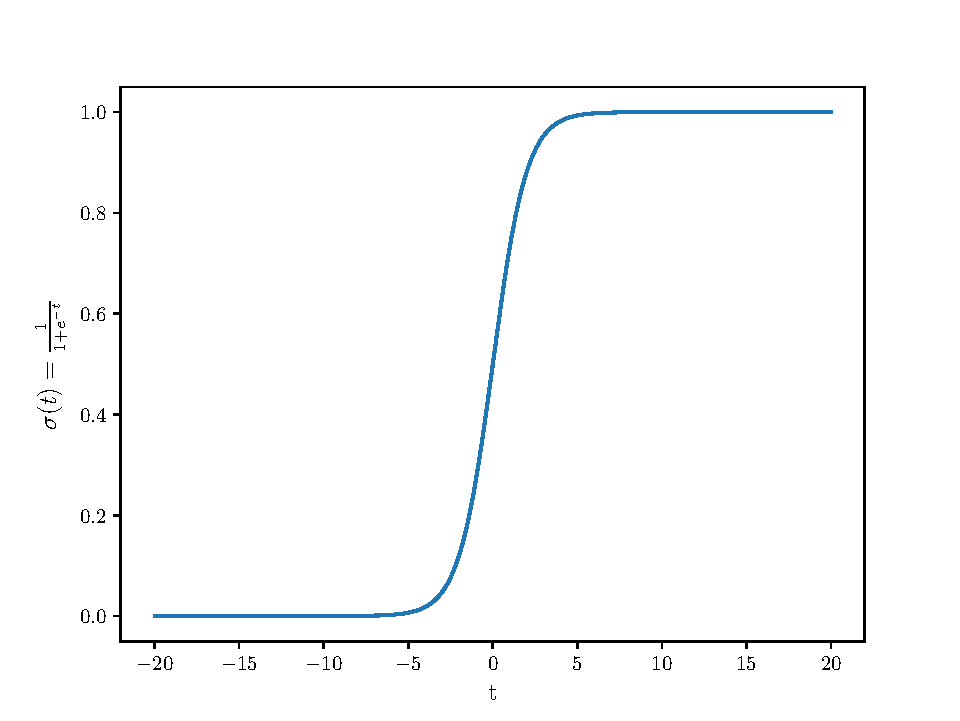
\includegraphics[width=0.55\textwidth]{sigmoid.pdf}
\caption{M. Nikoli\'c, A. Ze\v cevi\'c, Machine learning, in preparation.}
\end{figure}
}

\frame{
\frametitle{Going probabilistic}
\begin{itemize}
\item This can be seen as probability
$$p_w(y=1|x)=\sigma(w\cdot x)$$
\item Therefore $$p_w(y|x)=\sigma(w\cdot x)^y(1-\sigma(w\cdot x))^{1-y}$$
\item How to choose parameters $w$?
\end{itemize}
}

\frame{
\frametitle{Maximal likelihood principle}
\begin{itemize}
\item Likelihood function:
$$\prod_{i=1}^N p_w(y_i|x_i)=\prod_{i=1}^N\sigma(w\cdot x_i)^{y_i}(1-\sigma(w\cdot x_i))^{1-y_i}$$
\item Negative log likelihood:
$$NLL(w)=-\sum_{i=1}^N[y_i\log \sigma(w\cdot x)+(1-y_i)\log (1-\sigma(w\cdot x))]$$
\item Loss used is called {\em crossentropy} and is very common in classification tasks:
$$L(p,q)=-\sum_{j}p(j)\log q(j)$$
\end{itemize}
}

\frame{
\frametitle{Learning problem}
\begin{itemize}
\item Learning problem is to minimize regularized negative log likelihood:
$$NLL(w)=-\sum_{i=1}^N[y_i\log \sigma(w\cdot x_i)+(1-y_i)\log (1-\sigma(w\cdot x_i))]+\lambda\|w\|^2_2$$
\item The problem is convex!
\item Usually optimized by Newton's method, but let's go for gradient descent!
\end{itemize}
}

\frame{
\frametitle{Gradient}
\begin{flalign*}
\hspace{-5mm}
\frac{\partial NLL(w)}{\partial w_j}&=-\sum_{i=1}^N\left[y_i\frac{\partial}{\partial w_j}\log \sigma(w\cdot x_i)+(1-y_i)\frac{\partial}{\partial w_j}\log (1-\sigma(w\cdot x_i))\right]+\lambda\frac{\partial}{\partial w_j}\sum_{i=1}^nw_i^2 &\\
&=-\sum_{i=1}^N\left[y_i\frac{\sigma(w\cdot x_i)(1-\sigma(w\cdot x_i))}{\sigma(w\cdot x_i)}x_{ij}-(1-y_i)\frac{\sigma(w\cdot x_i)(1-\sigma(w\cdot x_i))}{1-\sigma(w\cdot x_i)}x_{ij}\right]+2\lambda w_j &\\
&=-\sum_{i=1}^N\left[y_i(1-\sigma(w\cdot x_i))x_{ij}-(1-y_i)\sigma(w\cdot x_i)x_{ij}\right]+2\lambda w_j &\\
&=\sum_{i=1}^N\left[\sigma(w\cdot x_i)-y_i\right]x_{ij}+2\lambda w_j&\\
\end{flalign*}
}

\frame{
\frametitle{Gradient descent updates}
\begin{itemize}
\item Elementwise:
$$w_j\leftarrow w_j-\mu\sum_{i=1}^N\left[\sigma(w\cdot x_i)-y_i\right]x_{ij}+2\lambda w_j$$
\item Matrix form:
$$w\leftarrow w-\mu X^T\left[\sigma(Xw)-y\right]+2\lambda w$$
\end{itemize}
}

\frame{
\frametitle{Unregularized vs. regularized}
\begin{figure}
\vspace{3mm}
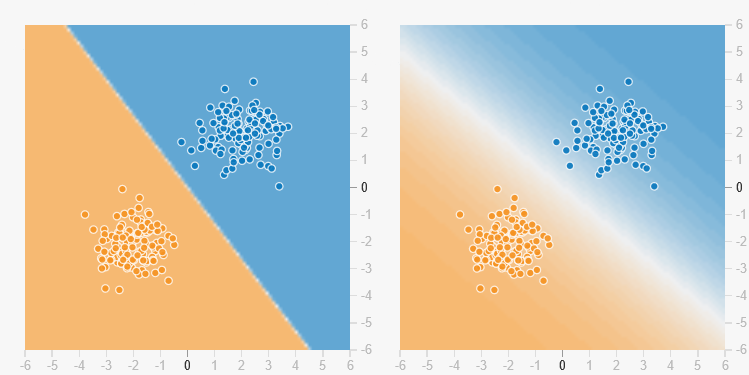
\includegraphics[width=0.7\textwidth]{logisticreg.png}
\caption{\url{https://playground.tensorflow.org}}
\end{figure}
}

\section{Basic preprocessing and evaluation}

\frame{
\frametitle{What is preprocessing?}
\begin{itemize}
\item Sometimes algorithms are not directly applicable to the data due to its form
\item Sometimes they are applicable, but their performance may be worse due to the form of the data
\item In such cases data needs to be transformed to a more desirable form, which is called {\em preprocessing}
\end{itemize}
}

\frame{
\frametitle{Some often used techniques}
\begin{itemize}
\item Coding of categorical features
\item Missing value imputation
\item Standardization/normalization
\item Outlier removal
\item Dimensionality reduction (e.g., PCA)
\item Decorrelation (e.g., PCA)
\item Aggregation of feature values or instances
\item Feature selection
\end{itemize}
}

\frame{
\frametitle{Dummy coding}
\begin{itemize}
\item How can we use a linear model if a categorical variable is present?
\item Consider a feature -- country of birth with $C$ possible outcomes
\item Terrible way to represent its values would be to, say, sort countries alphabetically and assign them indices in the sorted sequence
\item Meaningful way would be to introduce $C-1$ variables such that for $i$-th country all are $0$ except the $i$-th variable, which is 1 (for $i=C$, all are $0$)
\item Do not use $C$ variables with a linear model if bias term is included!
\item Prove that linear dependence of columns always happens in that case
\end{itemize}
}

\frame{
\frametitle{Missing value imputation}
\begin{itemize}
\item Sometimes, values of some variables are not observed, but the values of others are
\item One way of dealing with this problem is removing such instances, but they could be numerous
\item Such data also contains information which should be used
\item Two simple approaches:
\begin{itemize}
\item Imputation of the mean of observed values of the variable
\item Prediction of missing values by a regression model based on other variables
\end{itemize}
\end{itemize}
}

\frame{
\frametitle{Variables of different scale}
\begin{itemize}
\item Features are often measured at wildly different scales (e.g., savings and age)
\item If interpretability is of value, model parameters cannot be compared to determine relative importance of such variabels
\item Regularization will act differently on parameters corresponding to different variables
\item Numerical/optimization stability may be an issue
\end{itemize}
}

\frame{
\frametitle{Standardization}
\begin{itemize}
\item In response to the previous problem, some kind of feature scaling is virtually always applied
\item One such approach is standardization -- each feature is {\em centered} by removing the mean and divided by its standard deviation
\end{itemize}
}

\frame{
\frametitle{What does evaluation consist of?}
\begin{itemize}
\item Evaluation metrics -- metrics in which we express the quality of the model
\item Evaluation techniques  -- procedures used to compute metrics in a proper way
\end{itemize}
}

\frame{
\frametitle{Classifcation metrics}
\vspace{5mm}
\begin{itemize}
\item Often derived from confusion matrix
\end{itemize}
\begin{figure}
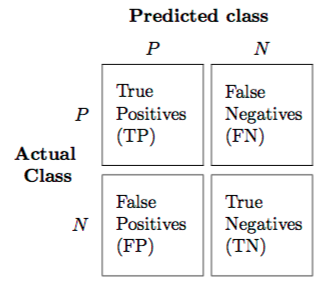
\includegraphics[width=0.47\textwidth]{confusion.png}
\vspace{-3mm}
\caption{MLxtend documentation}
\end{figure}
}

\frame{
\frametitle{Accuracy}
\begin{itemize}
\item Fraction of correctly classified instances among all classified instances
$$\frac{TP+TN}{TP+TN+FP+FN}$$
\item Sensitive to class imbalance
\item Consider detection of a rare disease
\end{itemize}
}

\frame{
\frametitle{AUC}
\begin{itemize}
\item Area under the (receiver operator characteristic) curve
\item The name is as ugly as a related interpretation (we focus on a nice one)
\item Assume that a binary classifier assigns a score to each class -- lower scores to class $0$ and higher scores to class $1$ (there should be a threshold)
\item Pick instances $x_0$ from class $0$ and $x_1$ from class $1$ at random
$$AUC=P(f_w(x_0)<f_w(x_1))$$
\item $0.5$ is random guessing and $<0.5$ means you are doing something very wrong :)
\item Insensitive to class imbalance
\end{itemize}
}

\frame{
\frametitle{Precision and recall}
\begin{itemize}
\item Often used in information retrieval and ranking
\end{itemize}
\begin{figure}
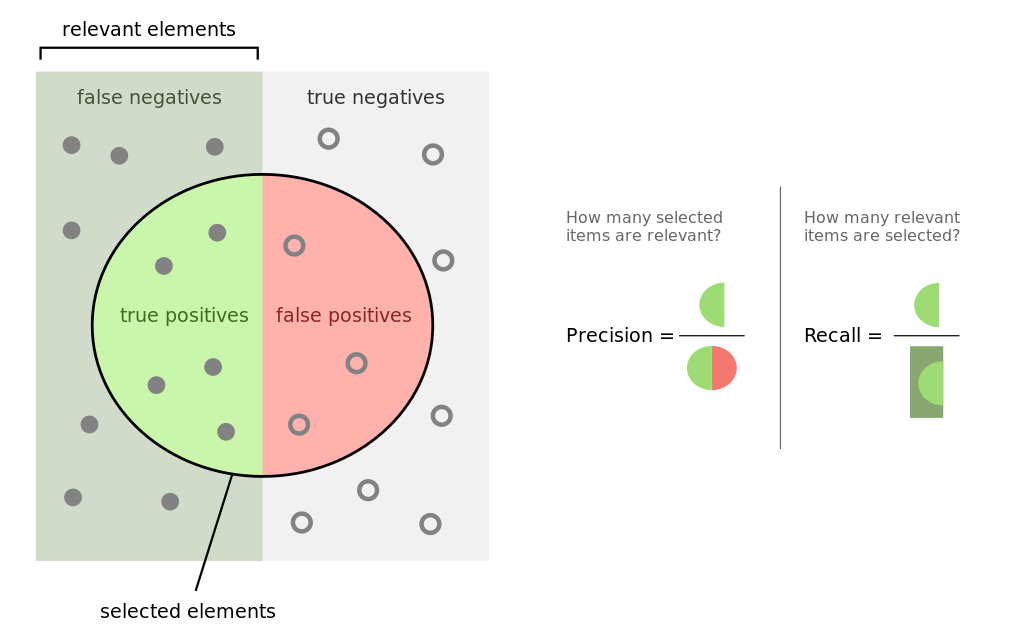
\includegraphics[width=0.71\textwidth]{precrec.png}
\vspace{-3mm}
\caption{https://en.wikipedia.org/wiki/Precision\_and\_recall}
\end{figure}
}

\frame{
\frametitle{Regression metrics}
\begin{itemize}
\item Often derived from model residuals
\end{itemize}
\begin{figure}
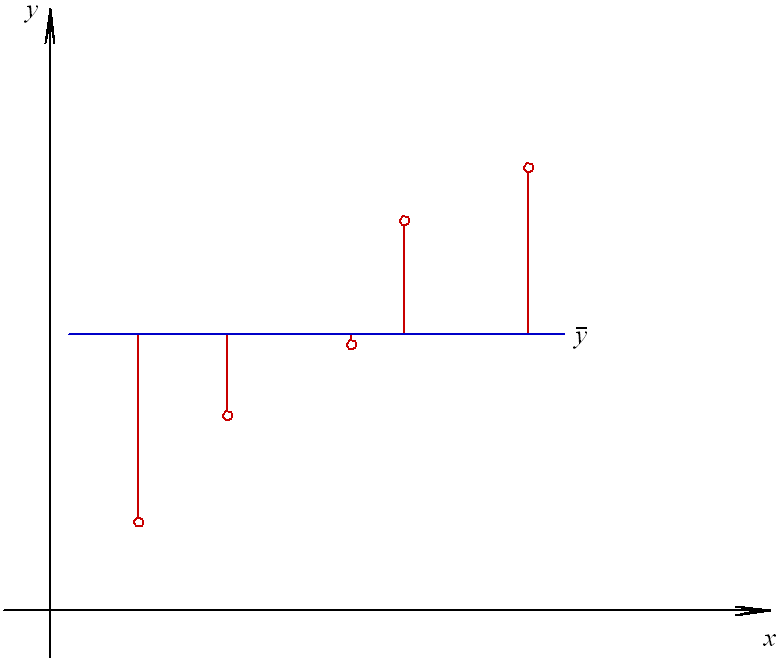
\includegraphics[width=0.5\textwidth]{razlikeprosek.png}
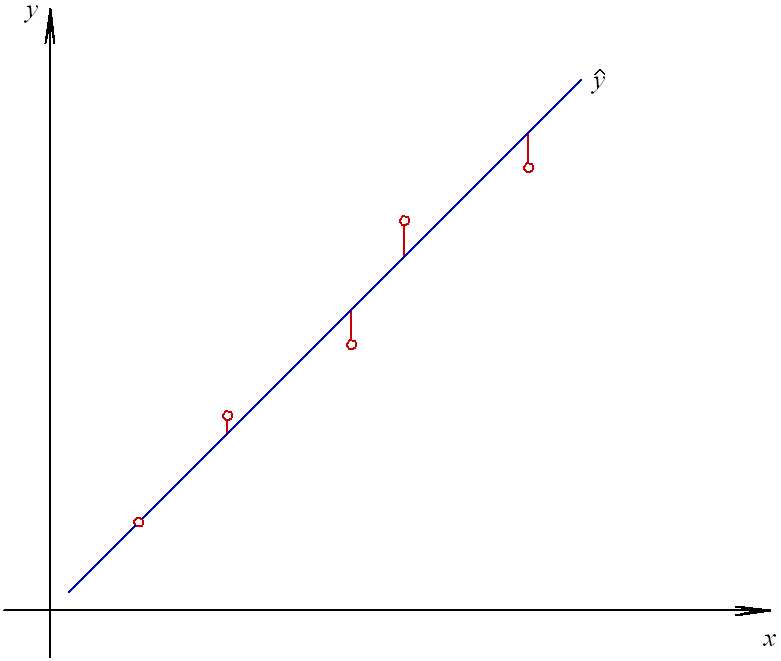
\includegraphics[width=0.5\textwidth]{razlikereg.png}
\vspace{-0.5mm}
\caption{P. Jani\v ci\'c, M. Nikoli\'c, Ve\v sta\v cka inteligencija, in preparation.}
\end{figure}
}


\frame{
\frametitle{Root mean squared error}
$$RMSE=\sqrt{\frac{1}{N}\sum_{i=1}^N(y_i-f_w(x))^2}$$
\begin{itemize}
\item Like standard deviation, but not with respect to the mean, but with respect to the model
\item Expressed in same units as the original variable
\item Used to estimate the magnitude of the error
\item Particularly useful if we know what magnitude of the error is acceptable in particular application
\end{itemize}
}

\frame{
\frametitle{Coefficient of determination $R^2$}
$$R^2=1-\frac{MSE}{Var}=1-\frac{\sum_{i=1}^N(y_i-f_w(x_i))^2}{\sum_{i=1}^N(y_i-\bar{y})^2}$$
\begin{itemize}
\item Measures the portion of variance of target variable explained by the model
\item In range $(-\infty,1]$
\item If $<0$ your training set is probably biased
\item More suitable in comparisons due to fixed scale
\end{itemize}
}

\frame{
\frametitle{Main tenant of model evaluation}
\begin{itemize}
\item Data used for model evaluation should by no means be used in its training!
\end{itemize}
}

\frame{
\frametitle{Training/testing split}
\begin{minipage}{0.49\textwidth}
\begin{itemize}
\item Split data into two sets -- training and test set
\item Use training set to train a model
\item Use test set to compute the error of the model
\item Used for a single training run (if there is such a thing), not for meta-parameter tuning!
\end{itemize}
\end{minipage}
\begin{minipage}{0.49\textwidth}
\begin{center}
\vspace{5mm}
\begin{tabular}{K{1cm}K{1cm}K{1cm}K{1cm}}
\hline
$x_1$ & $x_2$ & $x_3$ & $y$\\
\hline
\hline
\rowcolor{blue!50}
1 & 9 & 0 & 8\\
\rowcolor{blue!50}
0 & 6 & 2 & 1\\
\rowcolor{blue!50}
1 & 3 & 1 & 5\\
\rowcolor{blue!50}
4 & 9 & 7 & 6\\
\rowcolor{blue!50}
1 & 1 & 6 & 7\\
\rowcolor{blue!50}
7 & 2 & 3 & 4\\
\rowcolor{blue!50}
2 & 9 & 9 & 9\\
\rowcolor{red!50}
3 & 3 & 4 & 6\\
\rowcolor{red!50}
7 & 2 & 1 & 7\\
\rowcolor{red!50}
6 & 5 & 1 & 5\\
\end{tabular}
\end{center}
\end{minipage}
}

\frame{
\frametitle{Training/validation/testing split}
\begin{minipage}{0.69\textwidth}
\vspace{3mm}
\begin{itemize}
\item Split data into training, validation, and test sets
\item Tune the model by training it for different meta-parameter settings on the training and checking its performance on the validation set
\item Train on joint training and validation set using best meta-parameter values
\item Estimate the error of the best model on the test set
\end{itemize}
\end{minipage}
\begin{minipage}{0.29\textwidth}
\begin{center}
\vspace{5mm}
\begin{tabular}{K{1cm}K{1cm}K{1cm}K{1cm}}
\hline
$x_1$ & $x_2$ & $x_3$ & $y$\\
\hline
\hline
\rowcolor{blue!50}
1 & 9 & 0 & 8\\
\rowcolor{blue!50}
0 & 6 & 2 & 1\\
\rowcolor{blue!50}
1 & 3 & 1 & 5\\
\rowcolor{blue!50}
4 & 9 & 7 & 6\\
\rowcolor{green!50}
1 & 1 & 6 & 7\\
\rowcolor{green!50}
7 & 2 & 3 & 4\\
\rowcolor{green!50}
2 & 9 & 9 & 9\\
\rowcolor{red!50}
3 & 3 & 4 & 6\\
\rowcolor{red!50}
7 & 2 & 1 & 7\\
\rowcolor{red!50}
6 & 5 & 1 & 5\\
\end{tabular}
\end{center}
\end{minipage}
}

\frame{
\frametitle{Pitfalls of preprocessing and evaluation}
\begin{itemize}
\item No information from the test set should be used in training, therefore:
\begin{itemize}
\item For missing value imputation on the test set, use exclusively means computed on the training set
\item For standardization, use exclusively means and standard deviations computed on the training set
\end{itemize}
\item Test set selection should follow practically realistic scenarios
\end{itemize}
}

\section{Will It Work?}

\frame{
\frametitle{Will it work?}
\begin{center}
\LARGE{PROBABLY NOT!}
\end{center}
}

\frame{
\frametitle{If it's quite bad}
\begin{itemize}
\item Underfitting
\item Overfitting
\end{itemize}
}

\frame{
\frametitle{Underfitting vs. overfitting}
\vspace{0.6cm}
\begin{figure}
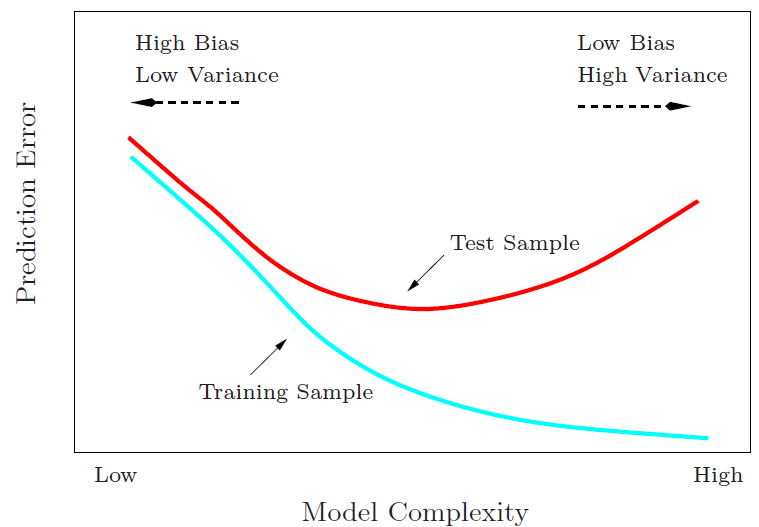
\includegraphics[width=0.615\textwidth]{biasvariance.png}
\caption{T. Hastie, R. Tibshirani, J. Friedman, ''Elements of Statistical Learning``, 2001.}
\end{figure}
}

\frame{
\frametitle{What if we have an underfitting problem?}
\begin{itemize}
\item Use more flexible models (even try to overfit)
\item Consider model properties -- maybe the one you used is not suited to the problem
\item Use lower regularization parameter values
\item Construct new features
\end{itemize}
}

\frame{
\frametitle{What if we have an overfitting problem?}
\begin{itemize}
\item Use less flexible models (even try to underfit)
\item Use feature selection
\item Use higher regularization parameter values
\item Use more data
\end{itemize}
}

\frame{
\frametitle{Word of caution}
\begin{itemize}
\item High training error and high test error indicate lack of flexibility which leads to underfitting
\item But not necessarily -- e.g., that could also happen due to large learning step
\item Low training error and high test error indicate too flexible model, which leads to overfitting
\item But not necessarily -- e.g., that could also happen due to bad preprocessing (stratification)
\item It's tricky, be cautious
\end{itemize}
}

\frame{
\frametitle{Sometimes it's all about features}
\begin{itemize}
\item If the features are not informative enough, no learning algorithm can help
\item Check which classes get mixed-up and check if existing features should be able to differentiate between them
\item Check for correlations between features and target variable
\item Consider using deep neural networks over raw data, instead of hand crafting the features
\end{itemize}
}

\frame{
\frametitle{Getting more into details}
\begin{itemize}
\item Check different error metrics, they tell you different things
\item If the model is interpretable, check if it makes sense
\item Check for patterns in instances for which the predictions are wrong
\item Inspect instances for which the model provides wrong answers with high confidence
\item Try to visualize errors -- might be easy for images, hard for high dimensional vectorial data
\end{itemize}
}

\frame{
\frametitle{Contact}
\begin{itemize}
\item Mladen Nikoli\'c\\ \url{nikolic@math.rs}
\item Machine Learning and Applications Group at the Faculty of Mathematics\\ \url{machinelearning.math.rs}
\end{itemize}
}

\frame{
\begin{center}
\LARGE{QUESTIONS?}
\end{center}
}

\end{document}
